%% Thermoelectric transport and spin filtering in hexagonal CrN nanoribbons
%% Elsevier elsarticle template -- target journal: Physica E
\documentclass[preprint,12pt]{elsarticle}

\usepackage{amsmath,amssymb}
\usepackage{graphicx}
\usepackage{booktabs}
\usepackage[hidelinks]{hyperref}
\usepackage{xcolor}

\graphicspath{{figures/}}
\journal{Physica E: Low-dimensional Systems and Nanostructures}

\begin{document}

\begin{frontmatter}

\title{Thermoelectric transport, spin filtering and thermal spin-valve operation in
hexagonal CrN nanoribbons: a tight-binding Landauer study}

\author[aff1,aff2]{Tomas Rojas\corref{cor1}}
\ead{tomas.rojas_s@ucr.ac.cr}
\author[aff3]{Ruhi Thorat}
\cortext[cor1]{Corresponding author}
\address[aff1]{Sede de Occidente, Universidad de Costa Rica, San Ram\'on, Costa Rica}
\address[aff2]{Centro de Investigaci\'on en Ciencia e Ingenier\'ia de Materiales (CICIMA),
Universidad de Costa Rica, San Jos\'e, Costa Rica}
\address[aff3]{Department of Physics and Astronomy, Ohio University, Athens, Ohio, USA}

\begin{abstract}
We present, to our knowledge, the first thermoelectric-transport study of hexagonal
(honeycomb) CrN nanoribbons. A tight-binding model fitted to published first-principles bands
of the half-metallic monolayer is combined with phase-coherent Landauer transport and a
phonon-Landauer thermal conductance, with no fresh ab-initio computation. Restoring the majority
conduction pocket that the minimal out-of-plane orbital manifold misses collapses the apparent
figure of merit of the zigzag $N{=}14$ ribbon from $ZT\simeq0.33$ to $0.06$ at $300$~K, a
basis-truncation artifact that parameter sensitivity cannot detect. With both majority
conduction bands and their anticrossing resolved, every optimum lies inside the fully
spin-polarized window: $ZT\simeq0.06$--$0.10$ at the onset of the second conduction band
($\mu-E_F\simeq+0.5$--$0.7$~eV) for five geometries, and $ZT=0.15$ ($0.08$--$0.24$ phonon
bracket) on the hole-doped side for the narrow armchair $N{=}8$ ribbon, the best case; the
minority band edge, where polarization is lost, is never the optimum. The ribbons
quantify, in the phase-coherent limit, the predicted perfect spin filtering: the minority
channel is gapped over nearly $4$~eV. A collinear antiparallel junction therefore switches
charge and heat currents off identically and acts as a thermal spin valve; a noncollinear
calculation shows that any continuous domain wall leaks (half transparency at $9$~\AA), so the
OFF state requires a constrained wall or nonmagnetic spacer. A self-consistent mean-field
treatment reproduces the magnetic edges and their exchange-coupling hierarchy.
\end{abstract}

\begin{keyword}
chromium nitride \sep nanoribbon \sep thermoelectric \sep half-metal \sep
Landauer transport \sep spin caloritronics
\end{keyword}

\end{frontmatter}

%% ------------------------------------------------------------------
\section{Introduction}
\label{sec:intro}

Low-dimensional thermoelectrics exploit quantum confinement to decouple the electrical and
thermal transport channels and to shape the electronic transmission near the Fermi
level~\cite{Hicks1993,Mahan1996}. Graphene, silicene, phosphorene and related nanoribbons have
therefore become a standard testbed for tight-binding plus Landauer studies of the Seebeck
coefficient and thermoelectric figure of merit~\cite{OuyangGuo2009,Sevincli2010}. Two ingredients
make magnetic nitride ribbons particularly interesting in this context: partially filled
transition-metal $d$ states, which generate sharp features in the density of states, and
intrinsically spin-polarized edges, which open the door to spin-caloritronic
functionality~\cite{Bauer2012}, namely thermally driven, magnetically switchable currents of the
kind predicted for ferromagnetic graphene~\cite{Zeng2011,Song2020} and
silicene~\cite{Ghanbari2018} nanoribbon junctions.

Chromium nitride is a prototypical correlated transition-metal nitride. In addition to its bulk
antiferromagnetic rock-salt phase, a freestanding two-dimensional hexagonal (honeycomb)
allotrope, $h$-CrN, has been predicted from first principles to be a $100\%$ spin-polarized
half-metallic ferromagnet with a large minority-spin gap and a magnetic moment of $3\,\mu_B$ per
Cr~\cite{Kuklin2017}. The monolayer has since been proposed, from first principles, as the basis
of lateral spin valves~\cite{Modarresi2019}. The finite-temperature magnetic order of the edges
of hexagonal CrN nanoribbons has been analyzed by density-matrix renormalization group (DMRG) in
a study that also computed spin-dependent semiclassical (Boltzmann) transport and
found the zigzag edges to act as perfect spin filters~\cite{CrNdmrg2023}; a one-dimensional
CrN nanostructure is likewise predicted to be a ferromagnetic half-metal~\cite{Xiang2023}, and
CrN thin films are experimentally established thermoelectric
materials~\cite{Quintela2009,Eklund2016,Sabeer2021}. Across all this activity, however, the
low-dimensional CrN literature is concerned with magnetism and spintronics; to our knowledge
the thermoelectric response has not been addressed.

Here we close this gap, with two purposes. First, we compute the phase-coherent, spin-resolved
Landauer transmission of hexagonal CrN armchair and zigzag nanoribbons
(Fig.~\ref{fig:geometry}) and evaluate the Seebeck coefficient, power factor, electronic thermal
conductance and figure of merit as functions of chemical potential, temperature, ribbon width,
edge type and spin channel. The approach is deliberately lightweight (a tight-binding model
parametrized from published band structures rather than a fresh ab-initio calculation), in
keeping with the analytic tradition of nanoribbon thermoelectrics and complementary, in both
property and method, to the DMRG study of Ref.~\cite{CrNdmrg2023}, which computes
spin-dependent semiclassical (Boltzmann) transport but no thermoelectric coefficients. Second,
we document a methodological pitfall of direct relevance to this tradition: the minimal orbital
manifold that suggests itself for $h$-CrN (the out-of-plane orbitals dominating the states at
$E_F$) omits the majority conduction band, an electron pocket at $K$, and thereby fabricates a
sharp transmission edge just above $E_F$ and a spuriously large figure of merit. We quantify
the artifact and show that no parameter-sensitivity analysis within the reduced
manifold can detect it.

\begin{figure*}[t]
\centering
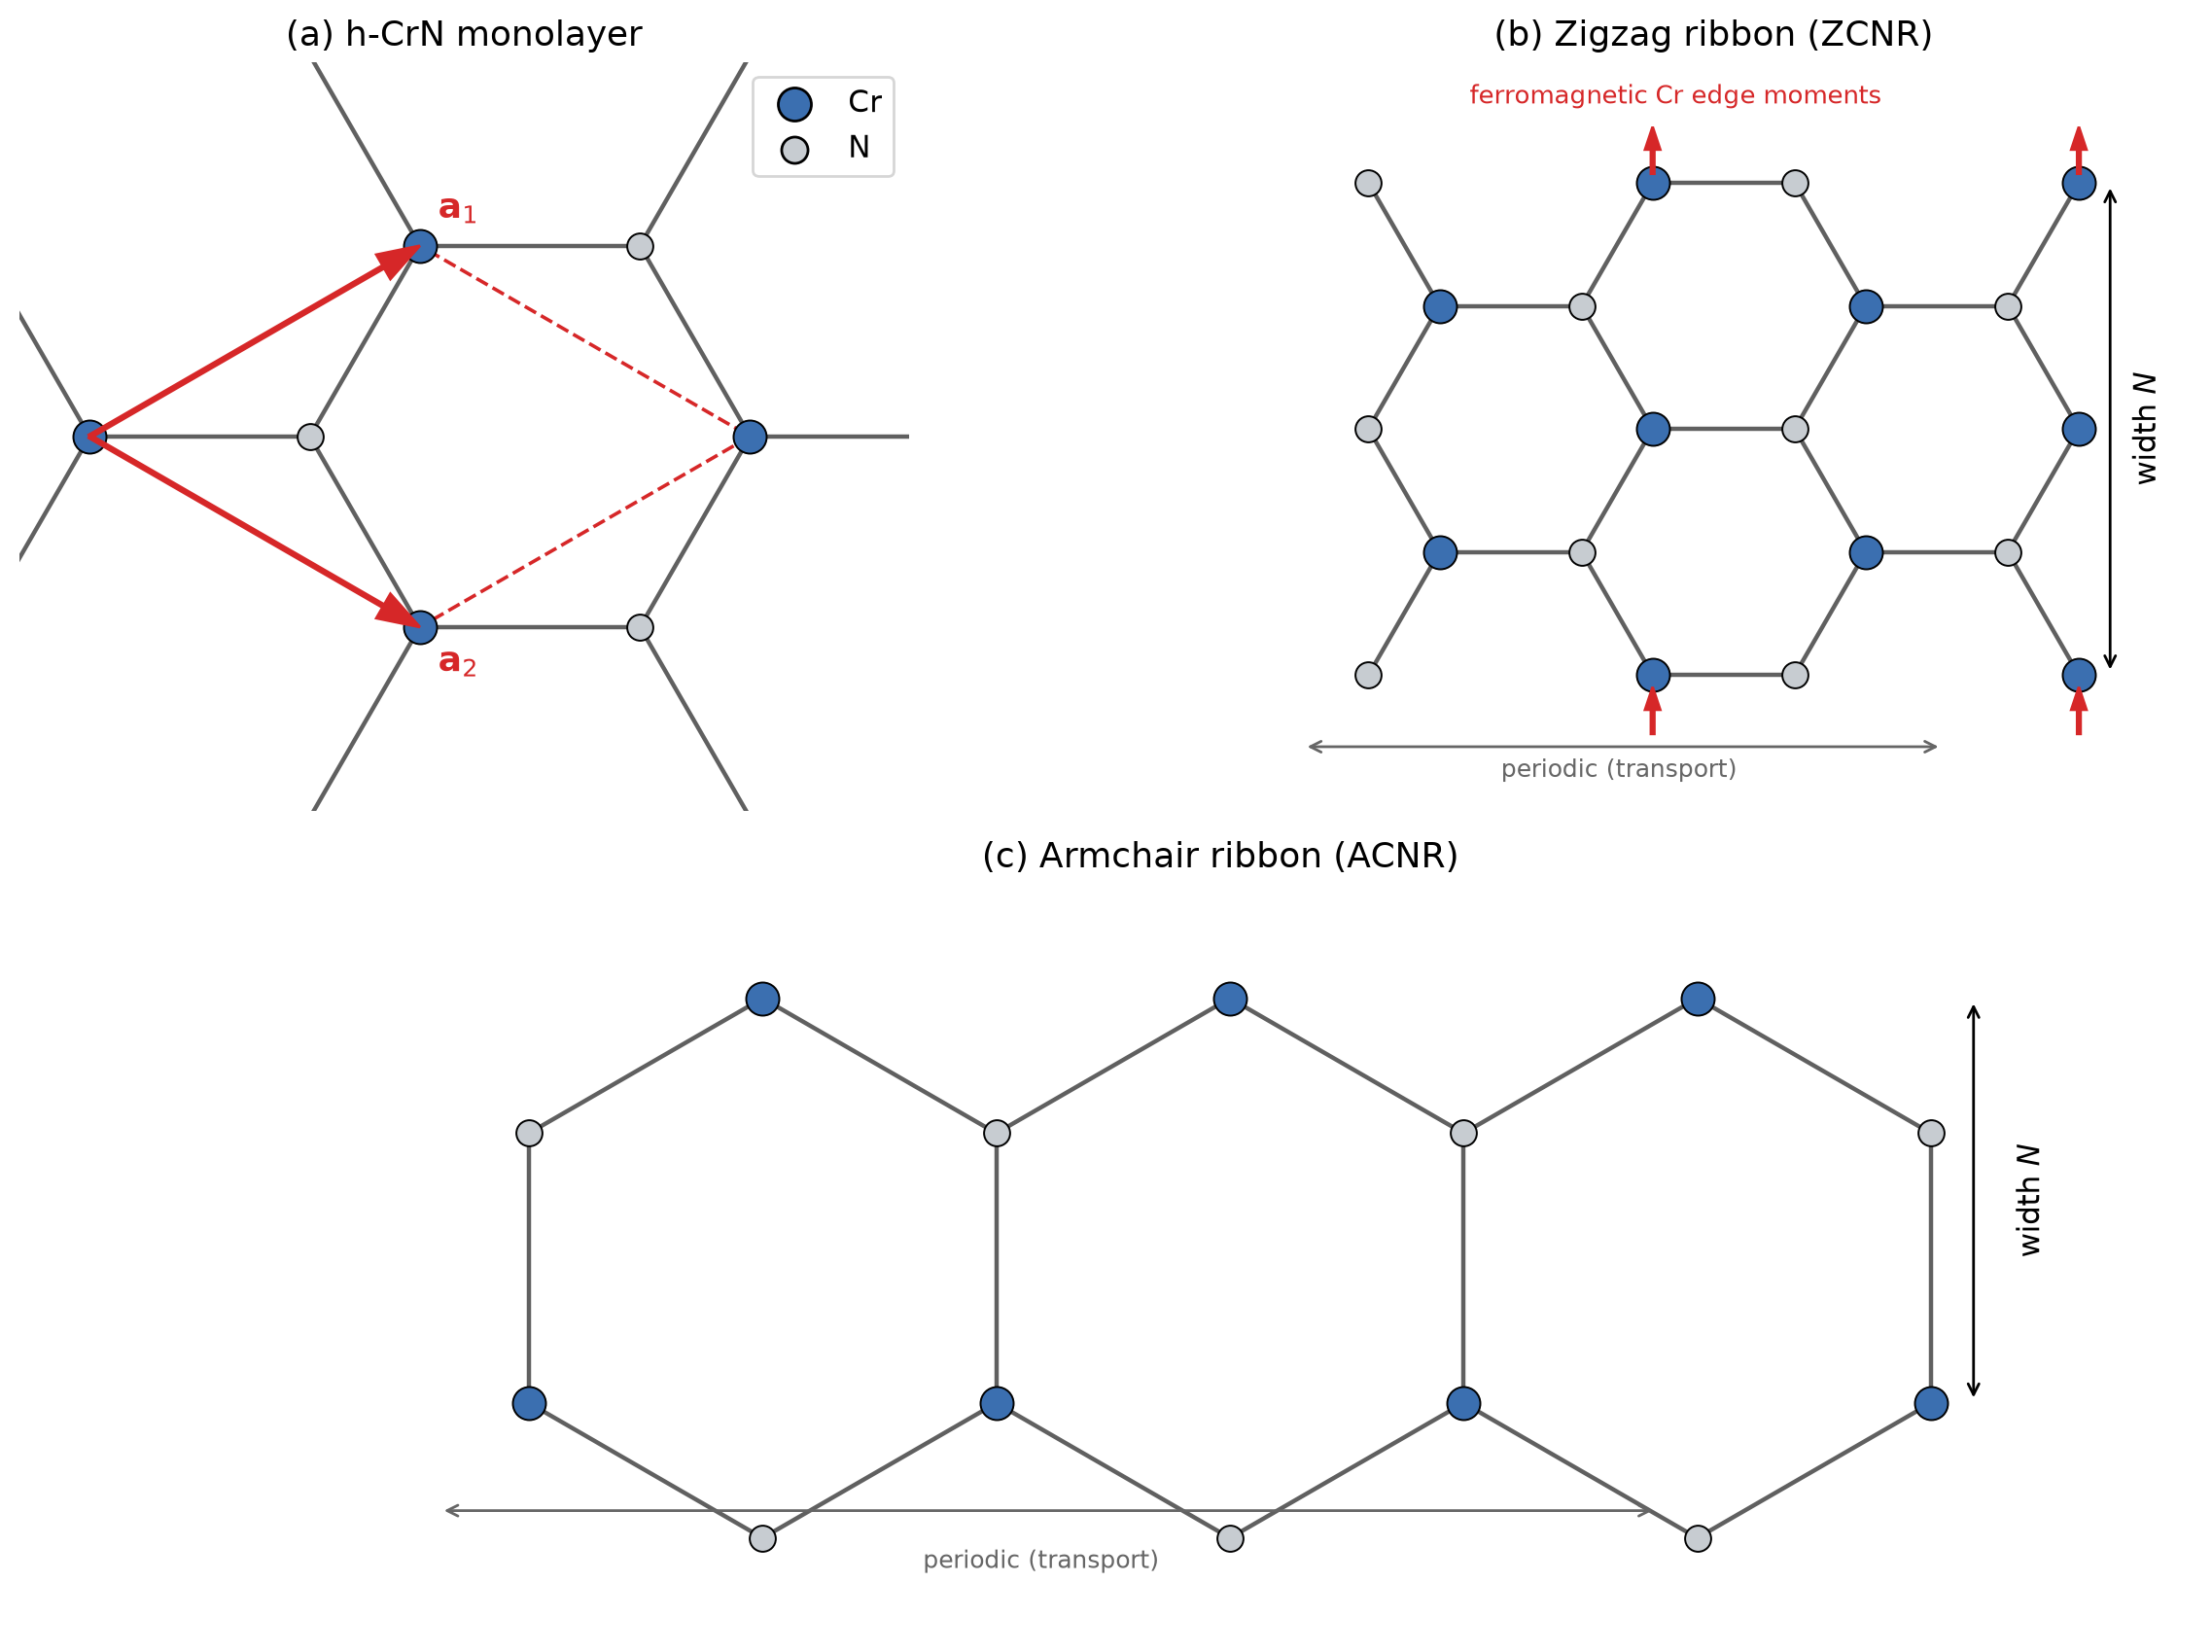
\includegraphics[width=0.9\textwidth]{fig1_geometry.png}
\caption{Geometry. (a) $h$-CrN monolayer honeycomb with Cr (blue) and N (gray) sublattices,
primitive vectors $\mathbf{a}_1,\mathbf{a}_2$ and unit cell. (b) Zigzag ribbon (ZCNR) with
ferromagnetic Cr edge moments; transport is along the periodic direction. (c) Armchair ribbon
(ACNR). The width index $N$, following Ref.~\cite{CrNdmrg2023}, counts the alternating Cr-only
and N-only atomic rows across the ribbon: $N=14$ means seven Cr and seven N
rows between the two edges.}
\label{fig:geometry}
\end{figure*}

%% ------------------------------------------------------------------
\section{Model and methods}
\label{sec:methods}

\subsection{Geometry and tight-binding Hamiltonian}
We consider the $h$-CrN monolayer, with Cr and N on the two triangular sublattices
[Fig.~\ref{fig:geometry}(a)], and cut armchair (ACNR) and zigzag (ZCNR) nanoribbons of width
$N$, defined as the number of Cr and N atomic rows across the ribbon
[Fig.~\ref{fig:geometry}(b,c)], following the convention of Ref.~\cite{CrNdmrg2023}. We use the
DFT lattice constant $a=3.258$~\AA\ and Cr--N bond length $1.884$~\AA~\cite{Kuklin2017}. The DFT
structure is very nearly planar (buckling $\pm0.071$~\AA~\cite{Kuklin2017}); we treat the sheet
as strictly planar, which makes the Slater--Koster selection rules below exact.

The states at $E_F$ derive from the out-of-plane orbitals~\cite{Kuklin2017}: we keep three Cr
orbitals ($d_{z^2},d_{xz},d_{yz}$) and the N $p_z$ orbital, with hoppings from the Slater--Koster
two-center integrals~\cite{SlaterKoster1954}. For an in-plane bond with direction cosines
$(l,m,0)$ the selection rules are transparent: N $p_z$ couples only to Cr $d_{xz},d_{yz}$
through $V_{pd\pi}$ (matrix elements $l\,V_{pd\pi}$ and $m\,V_{pd\pi}$), forming the
$\pi$-bonding and $\pi$-antibonding bands, while $d_{z^2}$ is non-bonding and disperses only
through a Cr--Cr second-neighbor hopping $t_{zz}$.

This out-of-plane manifold is, however, not sufficient: the reference band structure
[Ref.~\cite{Kuklin2017}, Fig.~2(d)] shows a majority conduction band with an electron pocket at
$K$ (minimum $-0.2$~eV) that rises through the entire window $0$--$2.4$~eV. Its weight comes
from orbitals outside the out-of-plane set (Cr $d_{xy},d_{x^2-y^2}$ and $s$ carry the
above-$E_F$ projected density of states~\cite{Kuklin2017}). A second majority conduction band
(CB2) enters the same window from above, with a minimum of $\simeq0.7$~eV at M and an
anticrossing with the first (CB1) between $\Gamma$ and M. We therefore add two effective
conduction orbitals $c_1,c_2$ on the Cr triangular sublattice, both symmetry-decoupled from
N~$p_z$ in the planar sheet, each with an on-site energy $\varepsilon_{c_i}$ and first- to
third-neighbor hoppings $t_{ci1},t_{ci2},t_{ci3}$, and coupled on site by a $k$-independent
$v_{12}$ that opens the anticrossing. Both bands were traced from a 300-dpi render of
Ref.~\cite{Kuklin2017}, Fig.~2(d), calibrated against the energy-axis labels (about 100 points
per band along $\Gamma$--M--K--$\Gamma$; estimated accuracy $\pm0.1$~eV in the transport window
and $\pm0.3$~eV near $\Gamma$, where the bands crowd), and the nine parameters were fitted
jointly by weighted least squares to the two lowest eigenvalues, with weights emphasizing the
transport window ($E<1.2$~eV). The traced points are plotted against the fitted bands in
Fig.~\ref{fig:bands} and are deposited, with the tracing and fit scripts, in the accompanying
repository. The rms residual in the transport window is $0.04$~eV (a single effective band
fitted to CB1 alone gives $0.17$~eV), smaller than the digitization uncertainty itself, so the
single-number uncertainty of the conduction bands in the transport window is $\sim$$0.1$~eV.
The fitted anticrossing gap is $0.13$~eV. Above $\simeq2.8$~eV, where CB2 leaves the traced
range, the upper band is unconstrained and rises to $\simeq7.5$~eV at $\Gamma$; this lies far
outside the transport window and has no consequence below.

The five $d$+$p_z$ parameters and the exchange splitting (Table~\ref{tab:params}) were adjusted
by hand (there is no automated objective function for them) to reproduce explicit targets
from Ref.~\cite{Kuklin2017}: the minority conduction-band edge at $+0.9$~eV
and valence-band edge at $-3.0$~eV, the majority conduction-pocket minimum at $K$ ($-0.2$~eV),
the majority $\pi^*$ valence band reaching $E_F$, and the non-bonding $d_{z^2}$ manifold at
$-2.5$ to $-2.0$~eV. The residuals of this fit are stated in Sec.~\ref{sec:results}, and
the sensitivity of every headline number to a $\pm10\%$ variation of each parameter is
quantified in Fig.~\ref{fig:sensitivity}.

The spin-resolved $6\times6$ Bloch Hamiltonian is block-diagonal in the orbital order
$(d_{z^2},d_{xz},d_{yz}\,|\,c_1,c_2\,|\,p_z)$,
\begin{equation}
H_\sigma(\mathbf{k})=
\begin{pmatrix}
H_d(\mathbf{k})+\Delta_\sigma & 0 & F(\mathbf{k})\\
0 & H_c(\mathbf{k})+\Delta^c_\sigma & 0\\
F^\dagger(\mathbf{k}) & 0 & \varepsilon_{p_z}
\end{pmatrix},\quad
H_c=\begin{pmatrix}\epsilon_{c_1} & v_{12}\\ v_{12} & \epsilon_{c_2}\end{pmatrix},
\label{eq:H}
\end{equation}
with $H_d=\mathrm{diag}(\varepsilon_{d_{z^2}}+t_{zz}S_1,\,\varepsilon_\pi,\,\varepsilon_\pi)$,
$F=V_{pd\pi}(0,\,f_{xz},\,f_{yz})^{\rm T}$ and
$\epsilon_{c_i}(\mathbf{k})=\varepsilon_{c_i}+\sum_n t_{cin}S_n(\mathbf{k})$, where
$S_n(\mathbf{k})=\sum_{\boldsymbol\tau_n}e^{i\mathbf{k}\cdot\boldsymbol\tau_n}$ runs over
the $n$-th shell of six Cr--Cr neighbors and
$f_{xz,yz}(\mathbf{k})=\sum_{\boldsymbol\delta}(\hat\delta_{x,y})
e^{i\mathbf{k}\cdot\boldsymbol\delta}$ over the three Cr--N bonds. The spin-dependent shift is
$\Delta_\uparrow=0$ and $\Delta_\downarrow=\Delta_{\rm ex}$ (and likewise
$\Delta^c_\uparrow=0$): the majority levels sit at their bare fitted positions and the minority
levels are rigidly raised, the convention used throughout this paper.

\subsection{Magnetism}
The monolayer is a uniform ferromagnet, so at mean-field (Stoner) level the on-site Hubbard term
on the Cr $d$ orbitals produces a rigid exchange splitting: the majority ($\sigma=\uparrow$)
levels are the reference and the minority ($\sigma=\downarrow$) levels are shifted up by
$\Delta_{\rm ex}$. We fix $\Delta_{\rm ex}$ from the reported minority band edges rather than
by solving the self-consistency for the uniform sheet. The mapping is transparent in the
model: the minority valence-band top is the bare N~$p_z$ level, reached at $K$ where the Cr--N
Bloch factor vanishes ($\varepsilon_{p_z}=-3.2$~eV), and the minority conduction-band minimum
is $\varepsilon_\pi+\Delta_{\rm ex}=+1.0$~eV. Of the two reported edges we target the
conduction edge ($+0.9$~eV~\cite{Kuklin2017}), to which the thermoelectric optimum is
pinned, at the stated $\sim$$0.1$--$0.2$~eV digitization accuracy; the model gap then comes
out $4.2$~eV rather than the reported $3.9$~eV because $\varepsilon_{p_z}$ lands at $-3.2$
instead of $-3.0$~eV, a residual on the far, transport-irrelevant side of the window. Because
the optimal doping tracks the minority conduction edge one-for-one, the quoted optimal $\mu$
values inherit the same $\sim$$0.1$--$0.2$~eV uncertainty (Sec.~\ref{sec:scope}). The
effective orbitals $c_1,c_2$ are assigned the same minority shift
($\Delta^c_\downarrow=\Delta_{\rm ex}$), consistent with their dominantly Cr-$d$ character;
their minority replicas then lie above $+3.3$~eV, far outside the transport window. The parameters
(Table~\ref{tab:params}) reproduce the half-metallic character, the non-bonding $d_{z^2}$
level below the valence-band top, the majority valence band that reaches $E_F$, and the
majority conduction pocket at $K$ ($-0.20$~eV in the model versus $-0.2$~eV in the DFT
reference). In the reduced $d$+$p_z$ manifold the Cr moment is $2.67\,\mu_B$, about $11\%$
below the reported $3\,\mu_B$, because the deeper $\sigma$-bonded orbitals, which also carry
moment, are not included; the conduction pocket adds a further $0.06$~electrons per cell to
the majority channel.

For the edge-magnetism analysis of Sec.~\ref{sec:edgemag} the rigid splitting is promoted to a
self-consistent one: an unrestricted mean-field interaction on the Cr $d$ orbitals in which the
minority levels on Cr site $i$ are shifted by $U_{\rm eff}\,m_i$, with $m_i$ the
self-consistent moment of that site (majority levels unshifted, as above). The Stoner parameter
$U_{\rm eff}=\Delta_{\rm ex}/m_{\rm Cr}=1.346$~eV is calibrated so that the uniform solution
reproduces the fitted bulk exchange ($m_{\rm Cr}=2.674\,\mu_B$ in the reduced manifold); the
filling is fixed at $N_e=4.717$ electrons per CrN cell, the filling of the fitted bulk bands at
$E_F=0$; and the loop iterates with linear mixing ($0.3$) to a tolerance of $10^{-4}\,\mu_B$ on
every site moment, using $60$ $k$ points in the one-dimensional ribbon Brillouin zone. The
nearly empty conduction orbitals are omitted from the self-consistency (together they hold
$\sim$$0.06$~e/Cr and contribute negligibly to the moments).

\begin{table}[t]
\centering
\caption{Model parameters (energies in eV, referenced to $E_F$). The $d$+$p_z$ parameters are
fitted by hand to the explicit band-structure targets of Ref.~\cite{Kuklin2017} listed in
Sec.~2.1; the nine conduction-orbital parameters are a joint weighted least-squares fit to the
two traced majority conduction bands of the same reference (traced points in
Fig.~\ref{fig:bands} and in the repository).}
\label{tab:params}
\begin{tabular}{lcl}
\toprule
Parameter & Value & Meaning \\
\midrule
$a$ & $3.258$~\AA & lattice constant \\
$\varepsilon_{d_{z^2}}$ & $-2.3$ & Cr $d_{z^2}$ on-site (majority) \\
$\varepsilon_{\pi}$ & $-2.6$ & Cr $d_{xz},d_{yz}$ bare on-site (majority) \\
$\varepsilon_{p_z}$ & $-3.2$ & N $p_z$ on-site \\
$V_{pd\pi}$ & $1.45$ & Cr($d_{xz,yz}$)--N($p_z$) hopping \\
$t_{zz}$ & $0.08$ & Cr--Cr first-shell ($d_{z^2}$) hopping \\
$\Delta_{\rm ex}$ & $3.6$ & exchange splitting of the Cr $d$ levels \\
$\varepsilon_{c_1}$ & $1.222$ & conduction orbital $c_1$ on-site (majority) \\
$t_{c11}$ & $0.326$ & $c_1$--$c_1$ first-shell hopping \\
$t_{c12}$ & $-0.093$ & $c_1$--$c_1$ second-shell hopping \\
$t_{c13}$ & $-0.021$ & $c_1$--$c_1$ third-shell hopping \\
$\varepsilon_{c_2}$ & $1.505$ & conduction orbital $c_2$ on-site (majority) \\
$t_{c21}$ & $0.548$ & $c_2$--$c_2$ first-shell hopping \\
$t_{c22}$ & $0.310$ & $c_2$--$c_2$ second-shell hopping \\
$t_{c23}$ & $0.149$ & $c_2$--$c_2$ third-shell hopping \\
$v_{12}$ & $0.066$ & on-site $c_1$--$c_2$ coupling (anticrossing) \\
$\Delta^c_{\downarrow}$ & $3.6$ & minority shift of $c_1,c_2$ (assumed $=\Delta_{\rm ex}$) \\
\bottomrule
\end{tabular}
\end{table}

\subsection{Landauer transport}
Semi-infinite leads are taken to be the pristine ribbon; the spin-resolved transmission
$T_\sigma(E)$ is obtained from the scattering matrix computed by the wavefunction-matching
algorithm implemented in Kwant~\cite{Groth2014kwant}. In the pristine limit $T_\sigma(E)$ counts
the propagating modes, so the transmission is quantized in integer steps
[Fig.~\ref{fig:transmission}]. All production transmissions are evaluated on a single energy
grid of spacing $5$~meV. Two checks control the numerics. First, the energy grid: the peak
$ZT$ of the zigzag $N{=}14$ ribbon at $300$~K is $0.0685$, $0.0632$, $0.0632$ and $0.0636$ for
grid spacings of $20$, $10$, $5$ and $2.5$~meV, so the production grid is converged to better
than $1\%$; at $100$~K the same quantity changes by $0.6\%$ between the two finest grids, so
the $ZT(T)$ curves below are converged down to $100$~K. Second, for a pristine ribbon the transmission is independent of the
scattering-region length by construction (leads and region are identical); we use this as a
numerical self-consistency check ($T_\sigma(E)$ computed for one to four unit cells agrees to
machine precision), not as a physical convergence statement. The length does matter for the
noncollinear domain-wall junctions of Sec.~\ref{sec:valve}, where the region is sized to
contain the wall. The convergence data are included in the repository.

\subsection{Thermoelectric coefficients}
The linear-response coefficients follow from the moments of the transmission weighted by the
Fermi window~\cite{SivanImry1986,CutlerMott1969,Datta1995},
\begin{equation}
L_n^\sigma(\mu,T)=\int\!\Big(\!-\frac{\partial f}{\partial E}\Big)\,(E-\mu)^n\,T_\sigma(E)\,dE ,
\end{equation}
with $f$ the Fermi function. Per spin channel the electrical conductance is $G=(e^2/h)L_0$, the
Seebeck coefficient $S=-(1/eT)L_1/L_0$, the electronic thermal conductance
$\kappa_e=(1/hT)(L_2-L_1^2/L_0)$ and the power factor $\mathrm{PF}=S^2G$. The two spin channels
add as parallel conductors, $G=\sum_\sigma G_\sigma$,
$S=\sum_\sigma S_\sigma G_\sigma/\sum_\sigma G_\sigma$, and
$\kappa_e=\sum_\sigma\kappa_{e,\sigma}+T[\sum_\sigma G_\sigma S_\sigma^2-(\sum_\sigma G_\sigma
S_\sigma)^2/\sum_\sigma G_\sigma]$; the last (bipolar) term vanishes wherever one spin channel
is gapped. The figure of merit is
\begin{equation}
ZT=\frac{S^2 G\,T}{\kappa_e+\kappa_{\rm ph}} .
\end{equation}

\subsection{Phonon thermal conductance}
\label{sec:phonons}
The phonon contribution is estimated by a ballistic phonon-Landauer mode count anchored to the
published density-functional perturbation theory (DFPT) phonon dispersion of the freestanding
$h$-CrN monolayer [Ref.~\cite{Modarresi2019}, Fig.~4(a)], which we digitized along $\Gamma$--M
and $\Gamma$--K (estimated accuracy $\sim$$0.3$~THz). All six branches of the two-atom cell are
included. The in-plane acoustic branches are linear near $\Gamma$, with
$v_{\rm LA}\simeq8.5$ and $v_{\rm TA}\simeq4.3$~km/s, and reach zone-boundary frequencies of
$10.4$ and $5.4$~THz; the flexural ZA branch, quadratic near $\Gamma$ as in every 2D
crystal, is represented as $\nu=\alpha q^2$ with $\alpha\simeq44$~THz\,\AA$^2$ read from the
same dispersion, and crosses over to its zone-boundary maximum of $4.7$~THz. The three optical
branches run from $(13.7,\,13.2,\,16.85)$~THz at $\Gamma$ to $(7.2,\,10.8,\,15.1)$~THz at the
zone boundary. Each in-plane acoustic and optical branch is a monotone sine-form
interpolation between its anchors [$\nu(q)=\nu_{\rm max}\sin(\pi q/2q_{\rm ZB})$ for LA and
TA, whose low-$q$ slopes then reproduce the digitized velocities, a consistency check],
while ZA follows its quadratic form until it meets the corresponding sine curve
[$\nu_{\rm ZA}(q)=\min(\alpha q^2,\,\nu_{\rm max}\sin(\pi q/2q_{\rm ZB}))$]. All branches are
treated as isotropic,
with the zone-boundary radius $q_{\rm ZB}=1.20$~\AA$^{-1}$ averaged over the digitized
$\Gamma$--M ($1.11$~\AA$^{-1}$) and $\Gamma$--K ($1.29$~\AA$^{-1}$) directions. For a ribbon
of transverse width $W$ the number of propagating channels of branch $b$ at frequency $\omega$
is $M_b=(W/\pi)q_b(\omega)$, with $q_b(\omega)$ the iso-frequency radius, bounded below by the
four gapless ribbon modes~\cite{Rego1998}. Then
\begin{equation}
\kappa_{\rm ph}(T)=\frac{1}{2\pi}\int_0^\infty\! d\omega\,\hbar\omega\,
\frac{\partial n_B}{\partial T}\,M(\omega),
\label{eq:kph}
\end{equation}
which recovers the universal quantum $4\kappa_0(T)$, $\kappa_0=\pi^2k_B^2T/3h$, at low
temperature and saturates once all branches are populated ($T\gtrsim500$~K). At $300$~K this
gives $\kappa_{\rm ph}=0.6$--$1.7$~nW/K for the ribbons studied here ($W=10$--$32$~\AA),
which grows with width. This is a deliberately simple, transparent estimate (coherent ballistic
transport, no anharmonicity or edge roughness), so we report $ZT$ for $\tfrac12$, $1$ and
$2\times\kappa_{\rm ph}$ throughout. One further modeling choice deserves a caveat.
The low-frequency floor of four gapless modes follows the Rego--Kirczenow result for a
three-dimensional elastic beam (one dilatational, one torsional and two flexural branches),
whereas a strictly two-dimensional sheet supports only three gapless acoustic branches (LA, TA,
ZA), and it is not established that a fourth, beam-like torsional mode survives for a ribbon
cut from a planar 2D crystal. We therefore recomputed every entry of
Table~\ref{tab:results} with a three-mode floor (script in the repository): the
low-temperature limit becomes $3\kappa_0$ instead of $4\kappa_0$, $\kappa_{\rm ph}(300~{\rm K})$
decreases by $0.7$--$6\%$ (most for the narrowest ribbons), and the tabulated $300$~K figures
of merit rise by only $0.3$--$3.5\%$ (armchair $N=8$: $0.145\to0.150$), within the rounding of
Table~\ref{tab:results} and far inside its $\tfrac12\times$/$2\times$ bracket. We keep the
four-mode floor in the tabulated values; the choice is conservative for $ZT$.

%% ------------------------------------------------------------------
\section{Results and discussion}
\label{sec:results}

\subsection{Monolayer bands and ribbon transmission}
Figure~\ref{fig:bands} compares the fitted spin-resolved band structure of the $h$-CrN monolayer
with the digitized bands of Ref.~\cite{Kuklin2017}. The model reproduces the half-metal. The
majority channel is metallic: the $\pi$-antibonding valence band reaches $E_F$ and the
effective conduction band forms the electron pocket at $K$ ($-0.20$~eV). The minority channel
is gapped, with $E_F$ inside a $4.2$~eV gap spanning $[-3.2,+1.0]$~eV (reported: $3.9$~eV,
$[-3.0,+0.9]$~\cite{Kuklin2017}). The flat non-bonding $d_{z^2}$ band sits $\sim\!2.5$~eV
below $E_F$. Both majority conduction bands, including their anticrossing between $\Gamma$ and M, are
reproduced to within $\sim$$0.1$~eV throughout the transport window. The fit has one known
residual: the $\pi^*$ valence-band top sits at $+0.19$~eV at $K$, whereas the DFT band peaks
at $\simeq0$ \emph{inside} the $\Gamma$--M and K--$\Gamma$ intervals and dips to $-1.6$~eV at
$K$. This misfit matters: its spurious spectral weight in $[0,+0.19]$~eV sits within a few
$k_BT$ of several polarized-window optima of Table~\ref{tab:results}, and the ribbon mode
counts inside the half-metallic window inherit the full dispersion of this band, not only its
edge energies. We therefore probe the consequence directly with a \emph{$\pi^*$-pinned} variant
of the model, $\varepsilon_\pi\to\varepsilon_\pi-0.19$~eV together with
$\Delta_{\rm ex}\to\Delta_{\rm ex}+0.19$~eV, which lowers the majority $\pi^*$ manifold,
placing its top at the DFT value $\simeq0$, while leaving the minority conduction edge, and
hence the half-metallic window, unchanged (as a side effect the minority $d_{z^2}$ level rises
by the same $0.19$~eV). Section~\ref{sec:widths} quantifies the consequences of this
variant for every ribbon of Table~\ref{tab:results}.

\begin{figure}[t]
\centering
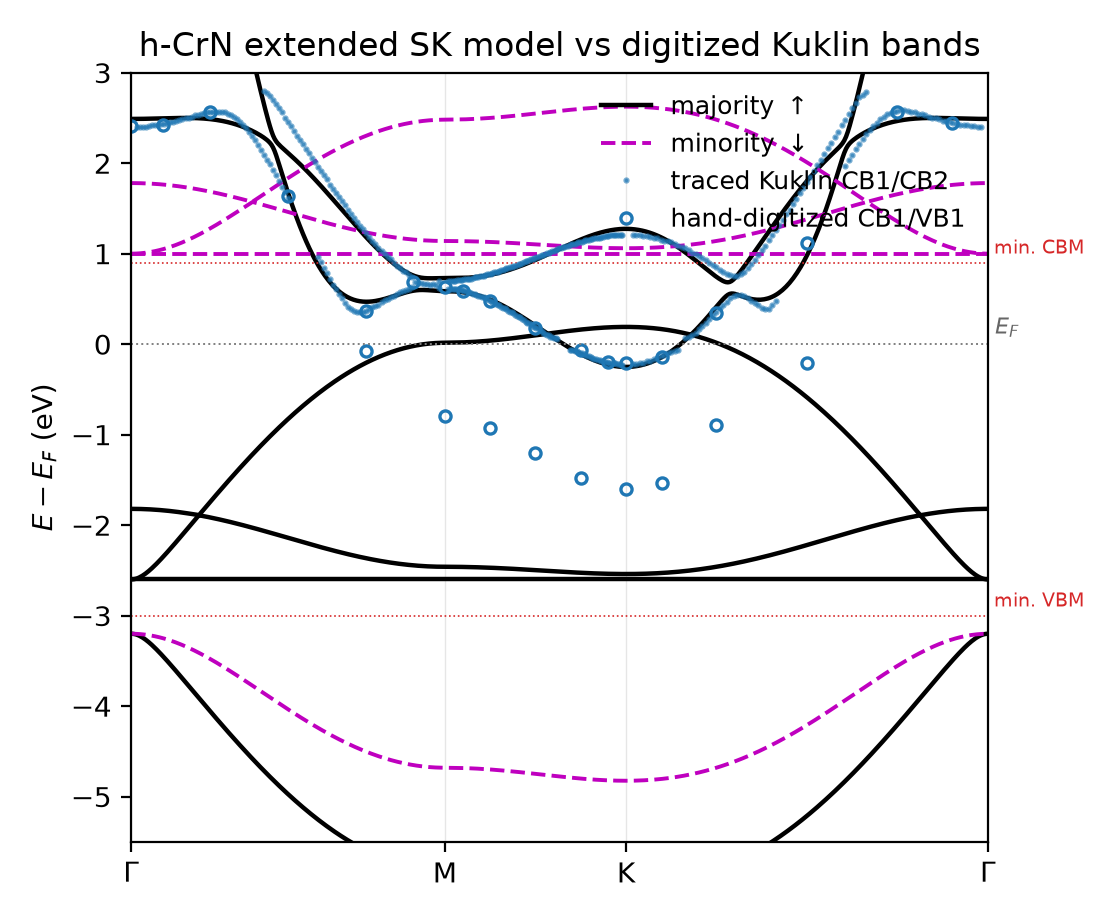
\includegraphics[width=0.8\columnwidth]{fig2_bands.png}
\caption{Spin-resolved tight-binding band structure of the $h$-CrN monolayer (majority: solid;
minority: dashed) compared with the digitized majority conduction band (CB1) and valence band
(VB1) of Ref.~\cite{Kuklin2017} (open circles) and the reported minority gap edges (dotted
lines). The majority channel is metallic (note the electron pocket at $K$) while the minority
channel is gapped across $E_F$: a half-metal.}
\label{fig:bands}
\end{figure}

Figure~\ref{fig:transmission} shows the spin-resolved transmissions of representative zigzag
and armchair ribbons. Both edges inherit the half-metallic character: the minority
transmission vanishes over the entire window $[-3.2,+1.0]$~eV while the majority channel
carries several quantized modes ($T_\uparrow(E_F)=8$ for zigzag $N=14$). The conductance
polarization $P_G=(G_\uparrow-G_\downarrow)/(G_\uparrow+G_\downarrow)$ is therefore $100\%$
for any chemical potential up to $\simeq+1.0$~eV: these ribbons are wide-window, gate-robust
spin filters. This confirms, in the phase-coherent limit, the spin filtering found for zigzag
edges by semiclassical transport~\cite{CrNdmrg2023}.

\begin{figure}[t]
\centering

\includegraphics[width=\columnwidth]{fig3_transmission.png}
\caption{Spin-resolved Landauer transmission $T_\sigma(E)$ of zigzag (left) and armchair (right)
CrN ribbons ($N=14$). The minority channel (dashed) is gapped over nearly $4$~eV around
$E_F$ while the majority channel (solid) conducts: the current is $100\%$ spin polarized up to
the minority conduction edge ($\mu-E_F\simeq+1.0$~eV), beyond which the conductance
polarization degrades (Sec.~\ref{sec:polar}).}
\label{fig:transmission}
\end{figure}

\subsection{The conduction pocket matters: a caution on minimal manifolds}
\label{sec:caution}
Figure~\ref{fig:manifold} quantifies the central methodological point. In the reduced
$d$+$p_z$ manifold the majority spectrum ends at $+0.19$~eV: the ribbon transmission drops
from several quanta to zero within $\sim$$0.2$~eV of $E_F$ and stays zero up to the minority
edge. That sharp edge is precisely what band-engineering
arguments~\cite{Hicks1993,Mahan1996} seek; it yields a large thermopower and a peak
$ZT\simeq0.33$ at $300$~K for the zigzag $N=14$ ribbon [Fig.~\ref{fig:manifold}(b)]. But the
edge is an artifact of basis truncation: with the conduction bands restored, majority modes
exist throughout the window, the transmission edge disappears, and the peak $ZT$ collapses by
a factor of five, to $0.063$, on the same phonon background. Varying every
retained parameter of the reduced manifold by $\pm10\%$ leaves the spurious result essentially
unchanged, because no variation of retained parameters can create a missing band. The caution
is generic rather than aimed at any published result. The standard single-$\pi$-orbital
workflow for graphene-family ribbons~\cite{OuyangGuo2009,Sevincli2010} is safe precisely
because no bands of other orbital character approach the operating window; a minimal basis
fitted only to the states at $E_F$ inherits this risk whenever the reference material, as is
typical for transition-metal compounds, has conduction (or valence) bands of different orbital
character within a few $k_BT$ of that window.

\begin{figure}[t]
\centering
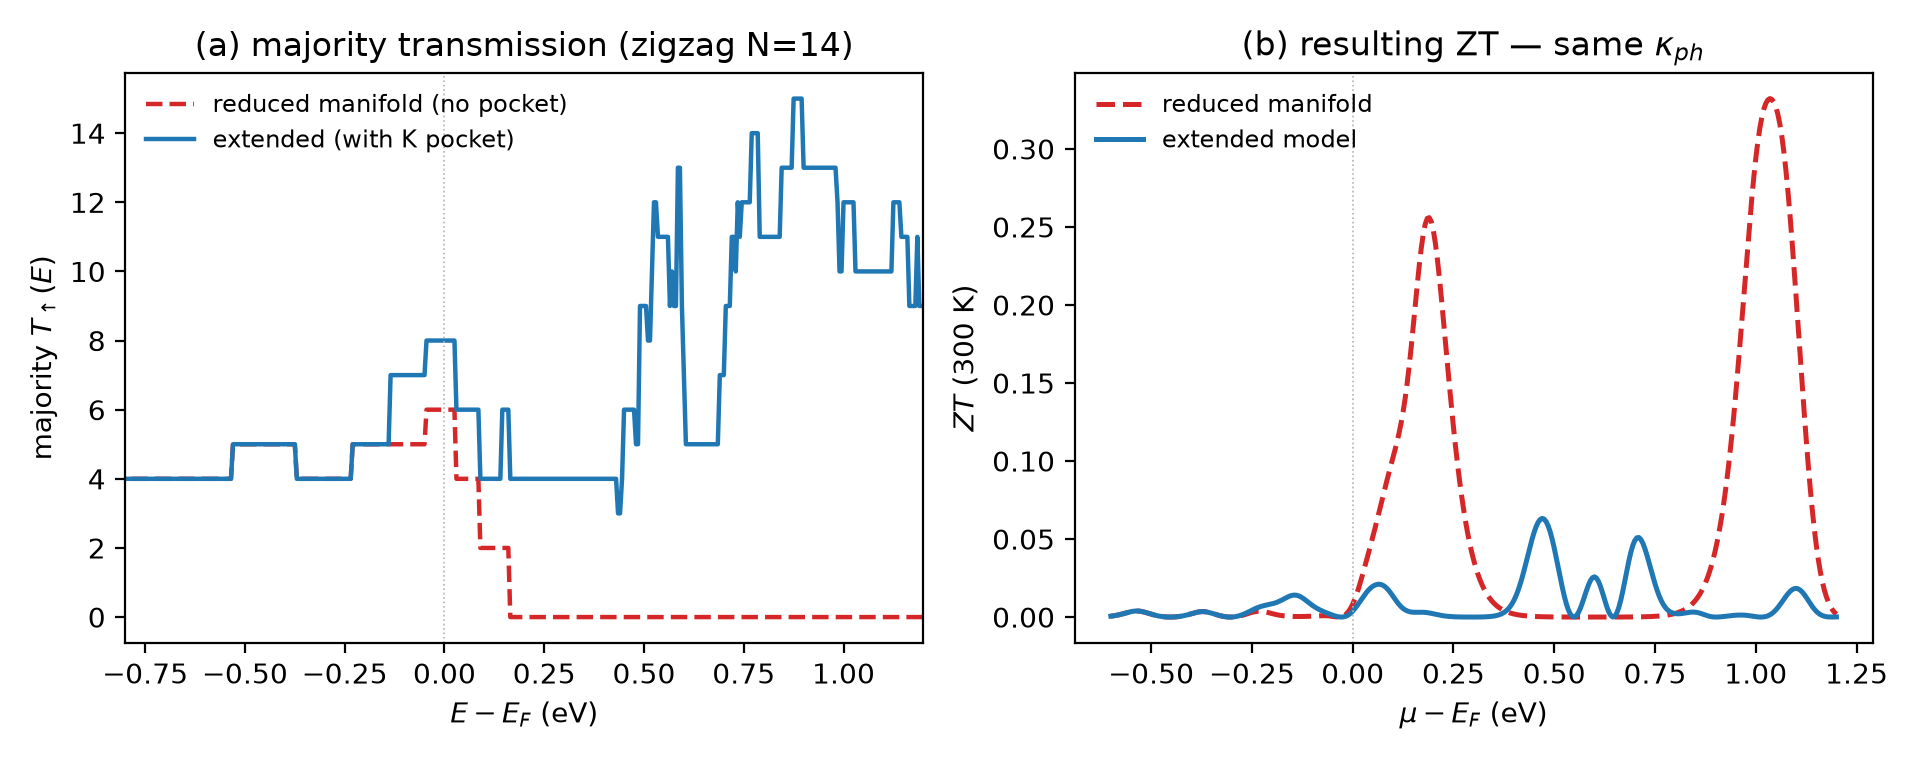
\includegraphics[width=\columnwidth]{fig_manifold.png}
\caption{Orbital-manifold caution (zigzag $N=14$, $300$~K). (a) Majority transmission in the
reduced $d$+$p_z$ manifold (dashed) and with the two effective conduction orbitals (solid):
the sharp edge above $E_F$ is an artifact of the truncated basis. (b) Resulting $ZT(\mu)$ on
the same phonon background: the apparent peak $ZT\simeq0.33$ collapses to $0.063$.}
\label{fig:manifold}
\end{figure}

\subsection{Seebeck coefficient, power factor and figure of merit}
\label{sec:te}
Figure~\ref{fig:spin}(a) shows the Seebeck coefficient of the zigzag $N=14$ ribbon. Within the
half-metallic window the majority background is metallic and multichannel, so $S$ is small and
oscillatory ($|S|\lesssim50$~$\mu$V/K at $300$~K) and changes sign as subband edges cross the
Fermi window. Two features stand out. The larger is at $\mu-E_F\simeq+0.5$~eV, where the
subbands of the second conduction band begin to enter: the majority mode count steps from
$6$ to $9$ within $0.25$~eV, giving $S\simeq-48~\mu$V/K with the minority channel still
closed, and the global maximum of the power factor and $ZT$ [Fig.~\ref{fig:zt}]. The second is
the minority edge at $\simeq+1.05$~eV, where the sharp minority onset supplies a large partial
thermopower ($S_\downarrow\simeq-150~\mu$V/K) against the smooth majority background
($S_\uparrow\simeq+9~\mu$V/K); because the majority channel now carries $13$ modes there, the
charge thermopower is only $\simeq-13~\mu$V/K and $ZT$ stays below $0.02$. For zigzag $N=14$
we obtain peak $ZT=0.063$ at $300$~K at $\mu-E_F=+0.47$~eV, with the $\tfrac12\times$/$2\times
\kappa_{\rm ph}$ bracket spanning $0.046$--$0.078$ [Fig.~\ref{fig:zt}(b)]. The
parameter-sensitivity spread is wider, $[0.029,0.114]$ (Sec.~\ref{sec:scope}); the two
brackets measure different things: phonon-model versus electronic-parameter uncertainty. At
the same doping $ZT$ is $0.067$ at $500$~K and $0.062$ at $700$~K, subject to the
magnetic-order caveat of Sec.~\ref{sec:scope}. These values are modest: in the coherent ballistic picture, pristine CrN
nanoribbons are not competitive thermoelectrics. They sit at the level of pristine graphene
nanoribbons in the same ballistic framework~\cite{OuyangGuo2009}; there, an order-of-magnitude
enhancement was achieved by edge disorder that suppresses phonons more strongly than
electrons~\cite{Sevincli2010}. We deliberately do not compute the electronic side of that
physics here: with the ballistic phonon background of Sec.~\ref{sec:phonons} held fixed,
disorder in the electronic channel alone can only degrade $ZT$, since the enhancement lives
entirely in the ratio of phonon to electron suppression. A meaningful disorder study requires
phonon transport through the same disordered geometry, which is outside the scope of this
model (Sec.~\ref{sec:scope}).

\begin{figure}[t]
\centering
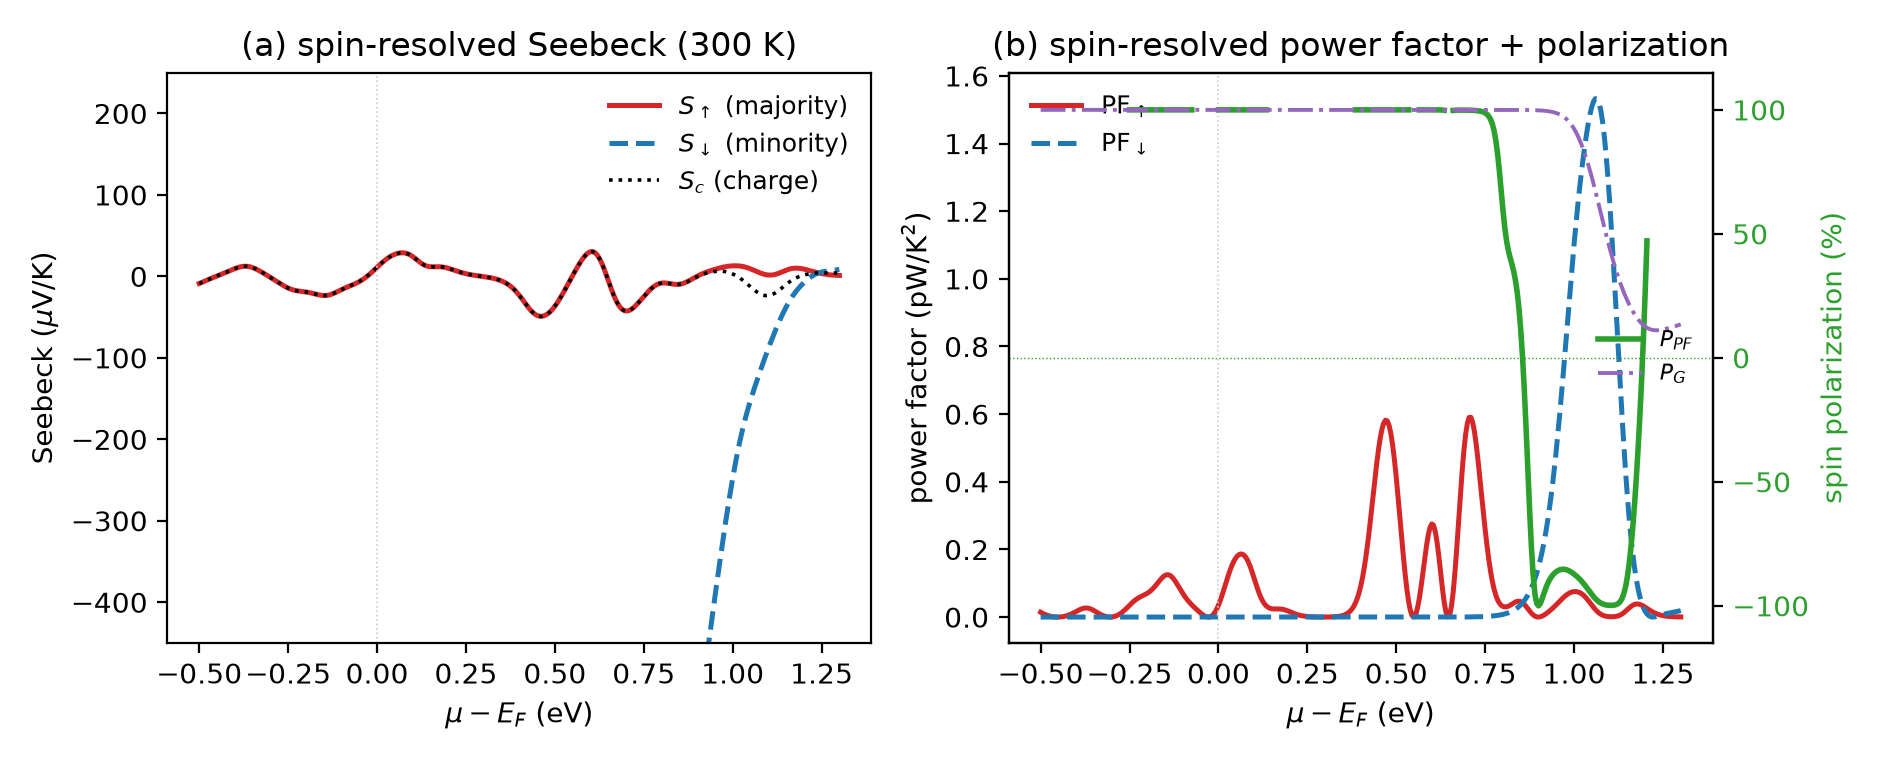
\includegraphics[width=\columnwidth]{fig_spinseebeck.png}
\caption{Spin-resolved thermoelectrics (zigzag $N=14$, $300$~K). (a) Spin-resolved Seebeck
coefficients $S_\uparrow$, $S_\downarrow$ and the charge thermopower $S_c$; each spin channel
is drawn only where its own conductance is non-negligible (deep in the minority gap
$S_\downarrow$ is exponentially activated and not meaningful). (b) Spin-resolved power
factors; right axis: conductance polarization $P_G$ (dash-dotted), which is $100\%$ across the
half-metallic window, and power-factor polarization
$P_{PF}=({\rm PF}_\uparrow-{\rm PF}_\downarrow)/({\rm PF}_\uparrow+{\rm PF}_\downarrow)$
(solid), which is undefined ($0/0$) and therefore masked where both power factors vanish
simultaneously (at sign changes of $S$); the gaps in the curve are not a loss of
polarization.}
\label{fig:spin}
\end{figure}

\begin{figure}[t]
\centering
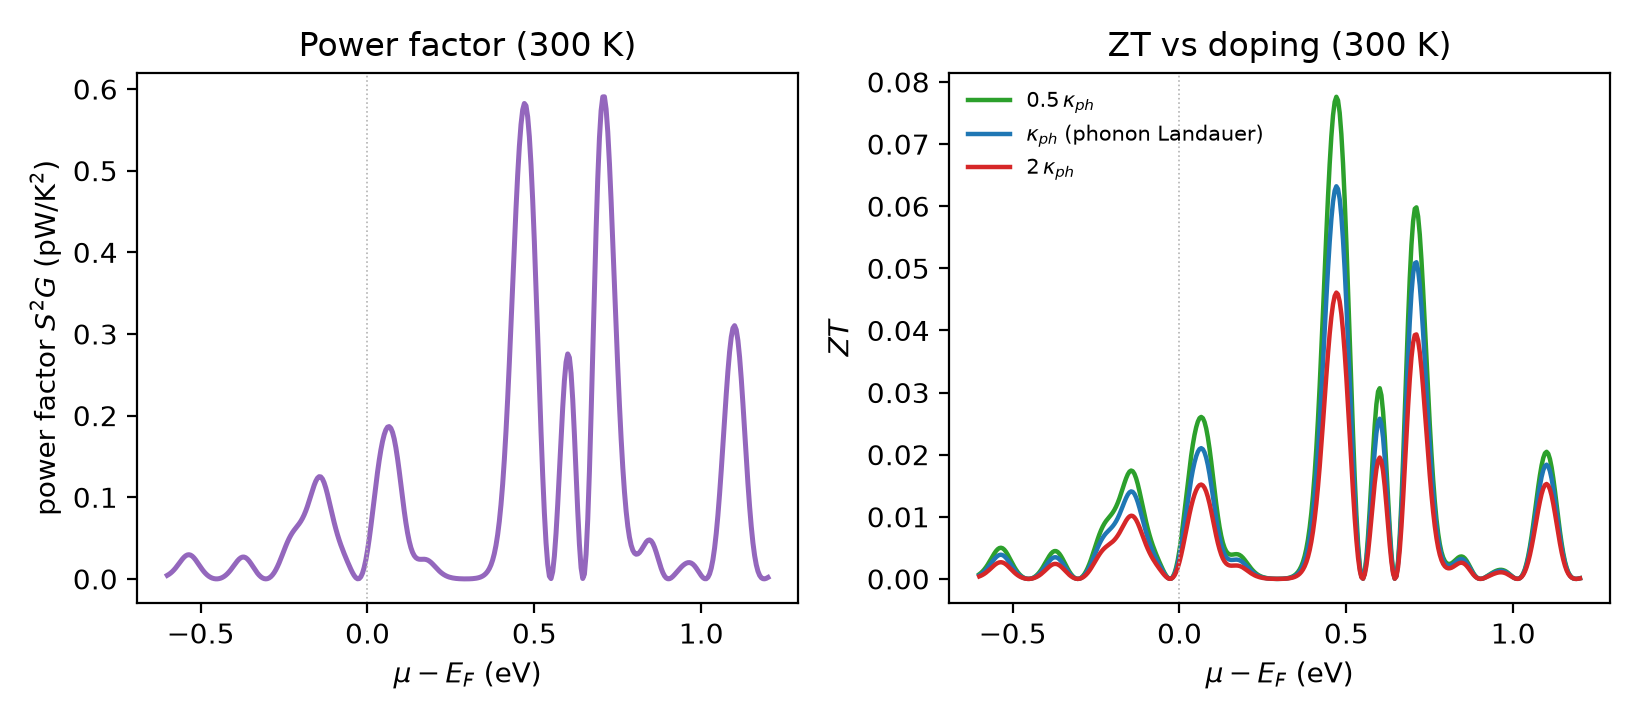
\includegraphics[width=\columnwidth]{fig5_zt.png}
\caption{(a) Power factor $S^2G$ versus doping at $300$~K (zigzag $N=14$): the maximum sits at
the onset of the second conduction band near $+0.7$~eV, inside the fully polarized window;
the minority edge near $+1.1$~eV is a weaker secondary feature. (b) $ZT$ versus doping for the
$\tfrac12\times$/$1\times$/$2\times$ $\kappa_{\rm ph}$ bracket.}
\label{fig:zt}
\end{figure}

\subsection{Width and edge dependence}
\label{sec:widths}
Table~\ref{tab:results} and Fig.~\ref{fig:designrules} collect the peak values for
$N=8,14,20$ and both edges, each ribbon with its own $\kappa_{\rm ph}(W)$ and
$\tfrac12\times$/$2\times$ bracket, and each optimum located by scanning
$\mu-E_F\in[-0.6,+1.2]$~eV, which covers the full minority gap and the metallic majority
background. Extending the scan to $-1.5$~eV (with $T(E)$ recomputed down to $-2.0$~eV; script
and data in the repository) changes no entry: on the $p$-type side ($\mu-E_F<-0.6$~eV) the
best value is $ZT\le0.03$ for every geometry, so ``global optimum'' below is global over
$[-1.5,+1.2]$~eV. Three observations replace the naive design rules that the reduced manifold would have
suggested.

(i)~Every global optimum lies inside the fully spin-polarized window. For five of the six
geometries it sits at the onset of the second conduction band ($\mu-E_F=+0.47$ to
$+0.71$~eV), where new majority subbands enter while the minority channel is still closed,
and reaches $ZT=0.06$--$0.10$; the minority edge ($+1.05$ to $+1.1$~eV), which dominated in a
model with a single conduction band, is now a secondary feature ($ZT\lesssim0.02$ for zigzag
$N=14$) because the second band supplies a large majority background there. Heavy electron
doping past the minority edge is therefore never the optimum, and the thermoelectric optimum
and full spin polarization coincide for every width and edge.

(ii)~$ZT$ does not grow with width: it is non-monotonic for both edges ($0.09$, $0.06$, $0.08$
for zigzag $N=8,14,20$; $0.15$, $0.07$, $0.10$ for armchair), because the subband spacing that
sharpens the transmission shrinks with $W$ while $\kappa_{\rm ph}$ grows with $W$, and the
two effects do not cancel monotonically. At matched width the armchair ribbon is better for
$N=8$ and $N=20$ and slightly worse for $N=14$.

(iii)~The narrow armchair $N=8$ ribbon remains the best geometry, shown in full in
Fig.~\ref{fig:armchair8}. Its optimum, $ZT=0.145$ $[0.082$--$0.235]$ at $300$~K, sits on a
majority subband feature at $\mu-E_F=-0.34$~eV ($S=-114$~$\mu$V/K), on the hole-doped side
and far from both conduction-band features. It is therefore insensitive to
$\Delta_{\rm ex}$ and to all nine conduction-orbital parameters, and the $\pm10\%$ sweep used
for the zigzag benchmark gives a strongly asymmetric spread: the optimum falls at most $7\%$
below the baseline ($0.135$), rises to at most $0.27$ (largest excursion $V_{pd\pi}$), and
stays inside the polarized window for every variation (for $\Delta_{\rm ex}{-}10\%$ and
$\varepsilon_{c_1}{+}10\%$ the second-conduction-band optimum at $\simeq+0.7$~eV overtakes it,
still fully polarized). Its $ZT$ decreases with temperature ($0.098$ at $500$~K, $0.088$ at
$700$~K), as do the second-conduction-band optima of the wider ribbons; only the narrowest
zigzag ribbon gains with temperature ($0.093\to0.106$ at $700$~K).

How much of this picture survives the model's known $\pi^*$ systematic? Recomputing every
entry of Table~\ref{tab:results} in the $\pi^*$-pinned variant of Sec.~\ref{sec:results}
changes no optimum: every peak value and position is identical to the baseline, except that
the armchair $N{=}8$ optimum shifts from $-0.34$ to $-0.45$~eV at unchanged $ZT=0.145$. The
reason is that the optima now sit on features of the conduction bands ($+0.5$ to $+0.7$~eV)
or, for armchair $N=8$, well below $E_F$, whereas the $\pi^*$ misfit affects only the
$[0,+0.19]$~eV interval; in the single-conduction-band model the same check had relocated
four of six optima. Rule~(i) is therefore robust against the one known systematic of the
fit, and the remaining uncertainty of the peak values is the parameter sensitivity of
Sec.~\ref{sec:scope}.

\begin{table}[t]
\centering
\caption{Peak figure of merit at $300$~K (global optimum over $\mu-E_F\in[-1.5,+1.2]$~eV;
every optimum lies inside the fully spin-polarized window $\mu-E_F<+1.0$~eV, where
$T_\downarrow=0$), each ribbon with its phonon-Landauer $\kappa_{\rm ph}(W)$; the ranges in
brackets are the $\tfrac12\times$/$2\times\,\kappa_{\rm ph}$ bracket. The last column is
$ZT$ at the same doping and $700$~K (ordered-phase transport, Sec.~\ref{sec:scope}). The
parameter-sensitivity spread (Sec.~\ref{sec:scope}) comes on top of the brackets. For
context, pristine graphene nanoribbons of comparable width reach similar values in the same
ballistic framework~\cite{OuyangGuo2009}.}
\label{tab:results}
\footnotesize
\setlength{\tabcolsep}{3pt}
\begin{tabular}{llcccc}
\toprule
Edge & $N$ & $W$ (\AA) & $\kappa_{\rm ph}$ (nW/K) & peak $ZT$ [$\tfrac12$--$2\times\kappa_{\rm ph}$] ($\mu{-}E_F$ [eV]) & $ZT$($700$~K) \\
\midrule
zigzag   & 8  & 10.2 & 0.62 & 0.093 [0.067--0.117] ($+0.48$) & 0.106 \\
zigzag   & 14 & 18.6 & 1.03 & 0.063 [0.046--0.078] ($+0.47$) & 0.062 \\
zigzag   & 20 & 27.1 & 1.46 & 0.083 [0.065--0.097] ($+0.71$) & 0.044 \\
armchair & 8  & 12.2 & 0.71 & 0.145 [0.082--0.235] ($-0.34$) & 0.089 \\
armchair & 14 & 21.9 & 1.19 & 0.072 [0.054--0.086] ($+0.71$) & 0.042 \\
armchair & 20 & 31.7 & 1.69 & 0.100 [0.074--0.121] ($+0.70$) & 0.053 \\
\bottomrule
\end{tabular}
\end{table}

\begin{figure*}[t]
\centering
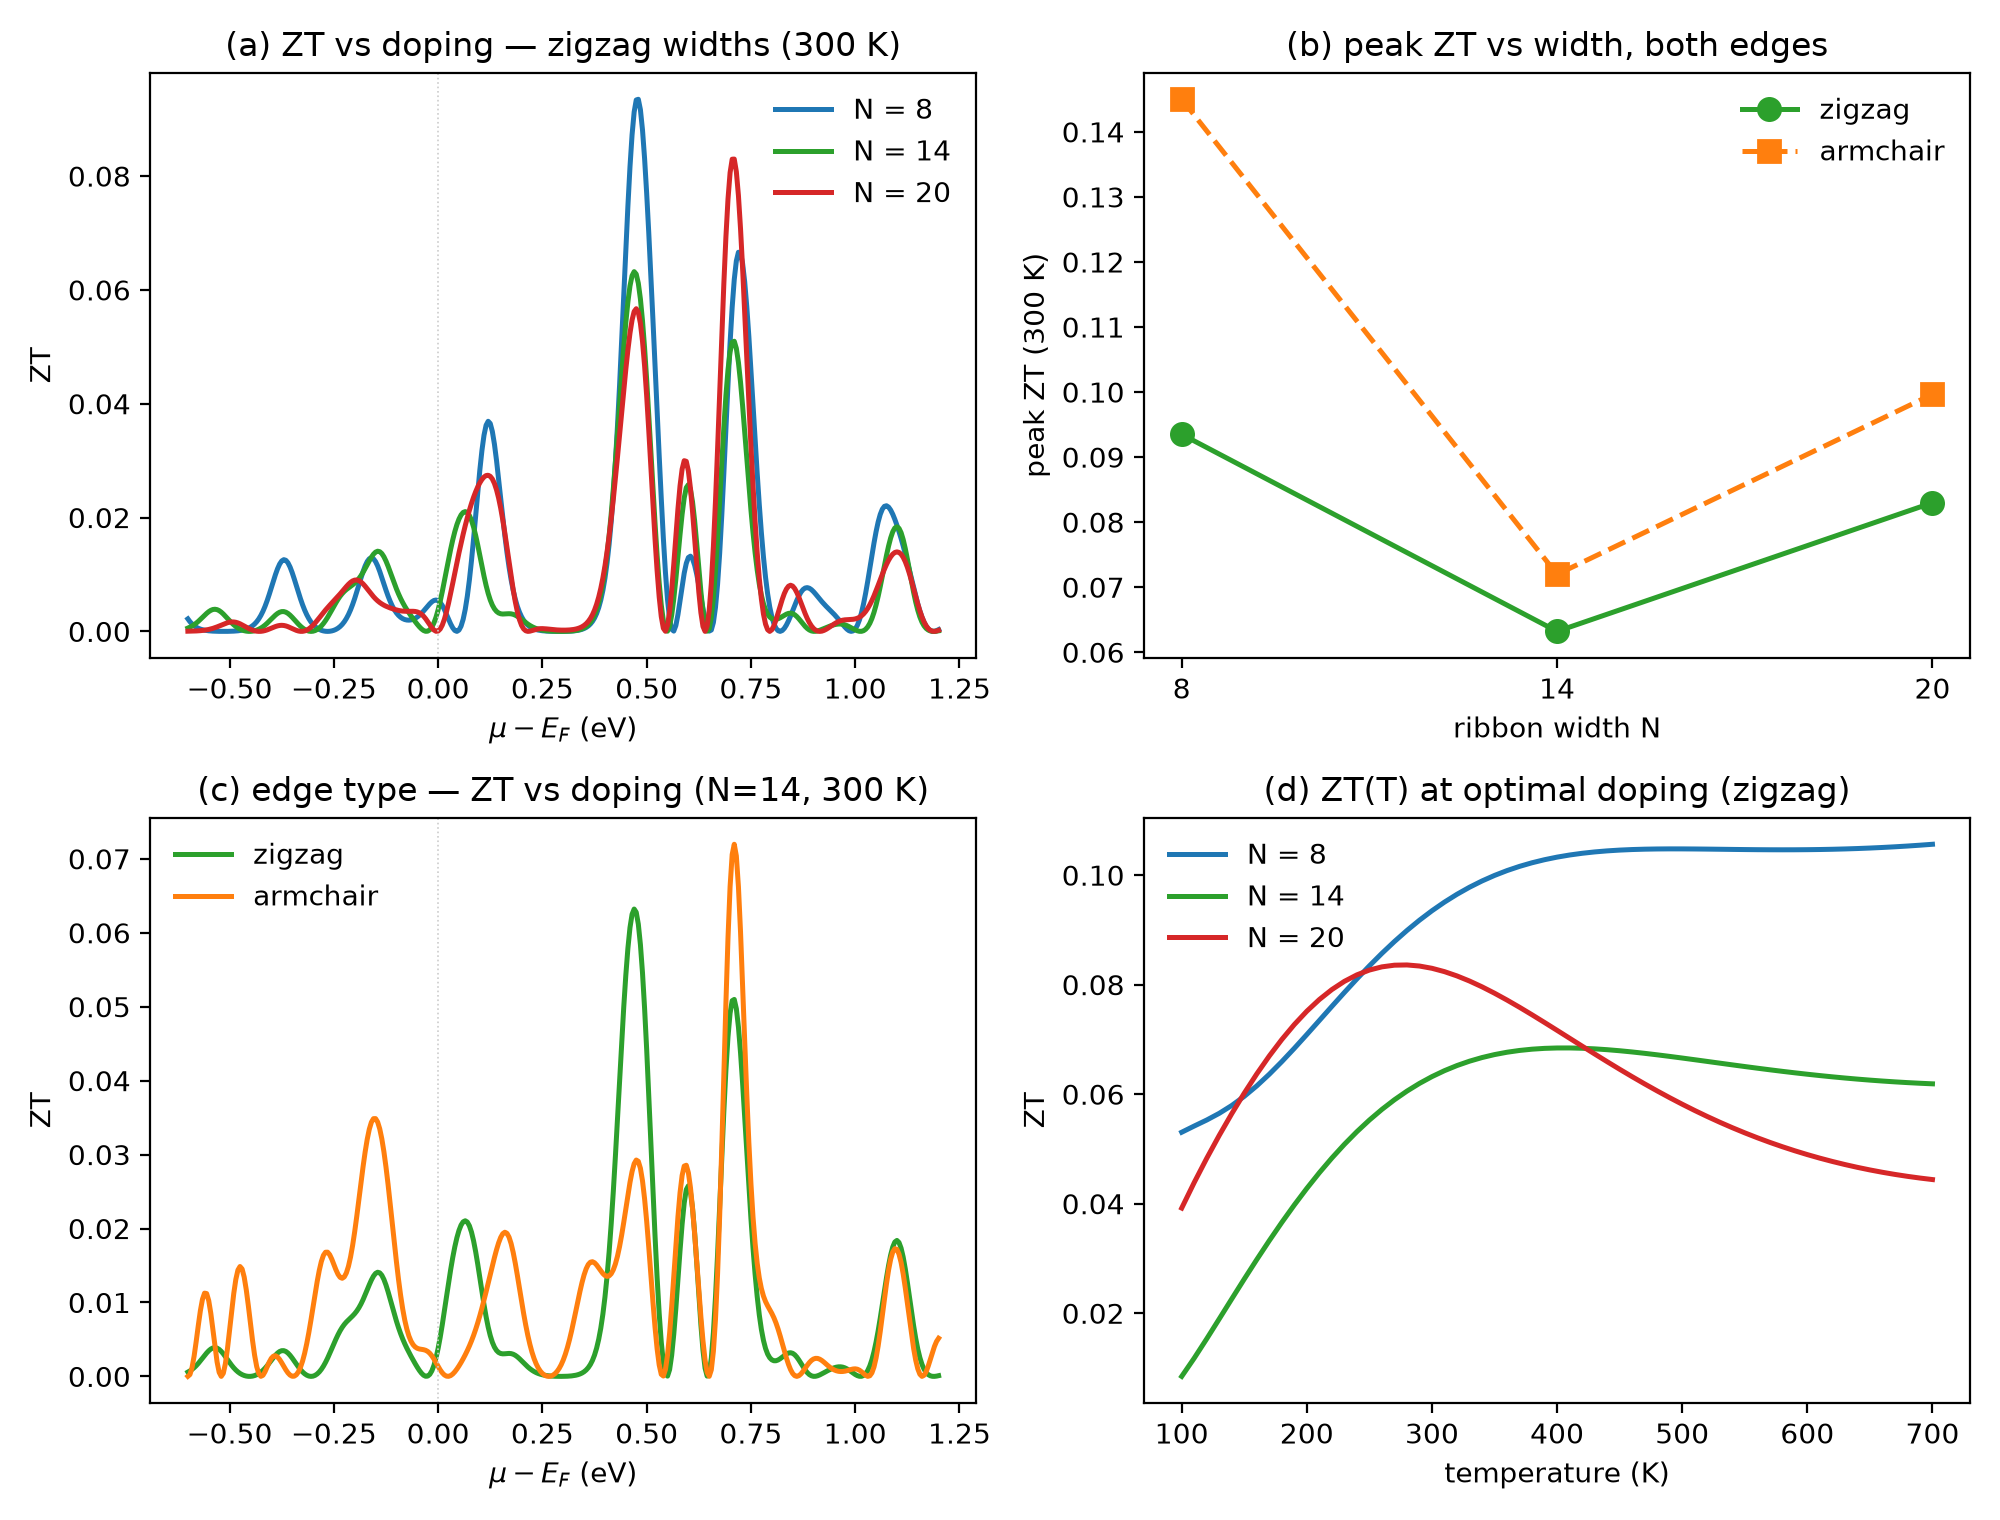
\includegraphics[width=\textwidth]{fig6_designrules.png}
\caption{Width, edge and temperature dependence. (a) $ZT$ versus doping for zigzag widths
$N=8,14,20$ at $300$~K, each with its own $\kappa_{\rm ph}(W)$. (b) Peak $ZT$ versus width for
both edge types. (c) Zigzag versus armchair at matched width $N=14$. (d) $ZT(T)$ at the $300$-K
optimal doping for the three zigzag widths (plotted from $100$~K, where the production grid
is converged to $<1\%$, Sec.~2.3).}
\label{fig:designrules}
\end{figure*}

\begin{figure*}[t]
\centering
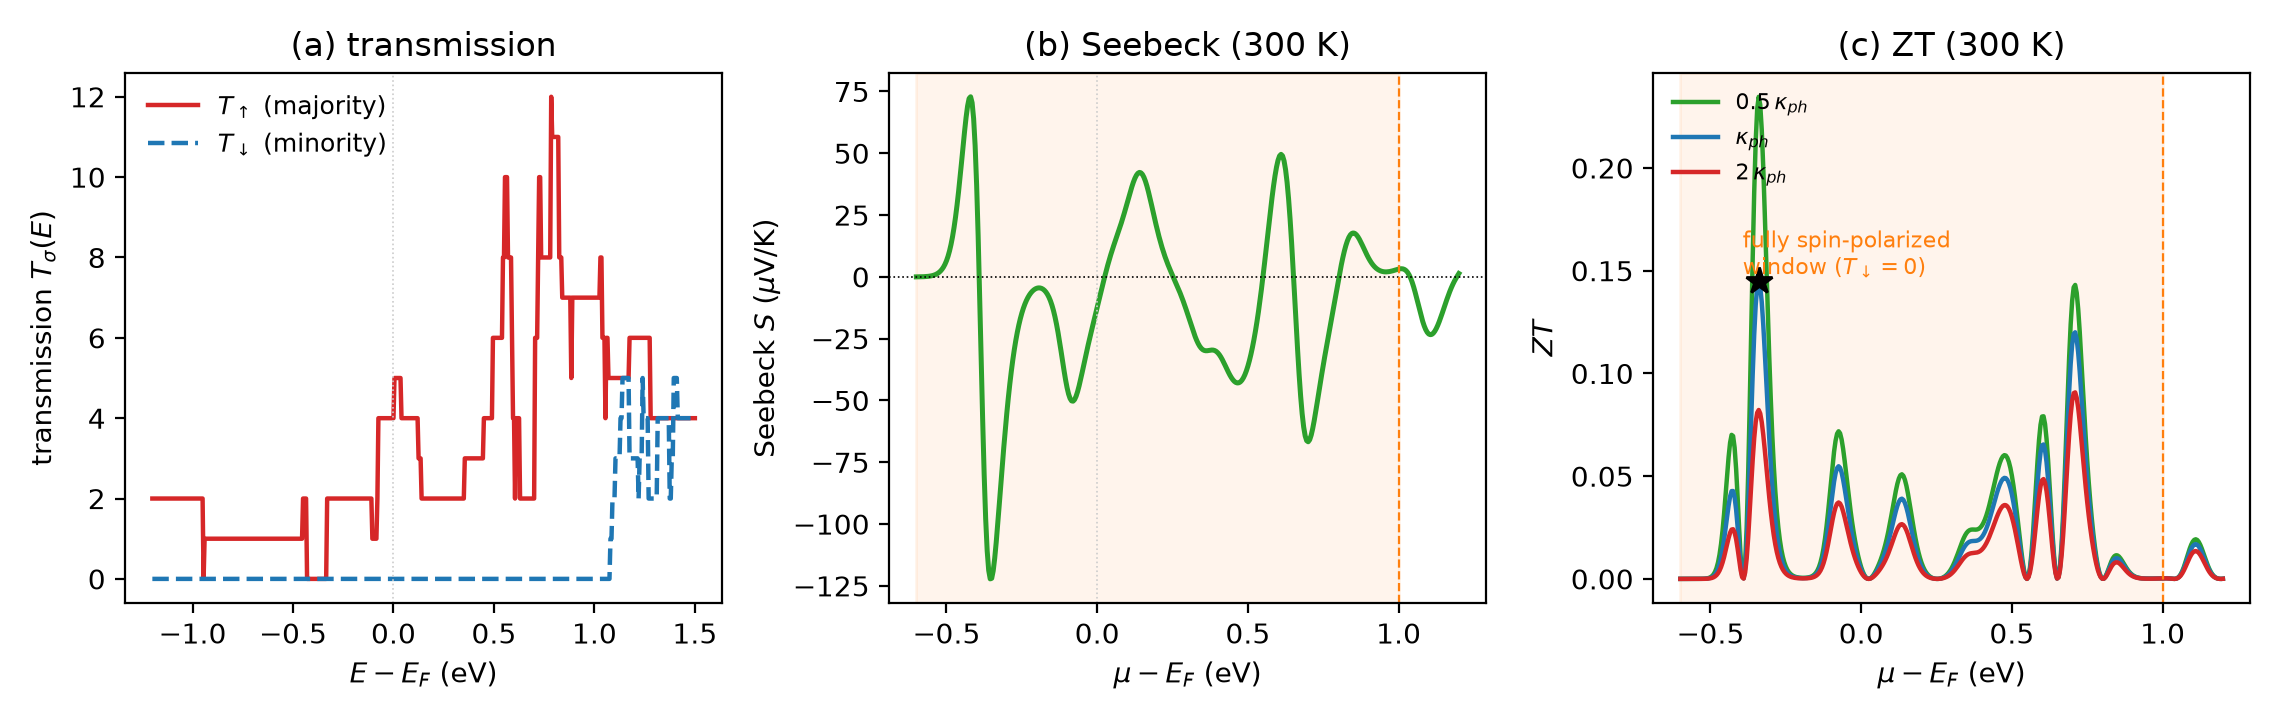
\includegraphics[width=\textwidth]{fig_armchair8.png}
\caption{The armchair $N=8$ ribbon, the best geometry; its optimum lies on the hole-doped side,
deep inside the fully spin-polarized window (shaded; minority edge dashed). (a) Spin-resolved
transmission. (b)
Charge Seebeck coefficient at $300$~K. (c) $ZT$ at $300$~K with the $\kappa_{\rm ph}$ bracket;
the star marks the optimum at $\mu-E_F=-0.34$~eV quoted in Table~\ref{tab:results}.}
\label{fig:armchair8}
\end{figure*}

\subsection{Spin caloritronics and a thermally driven spin valve}
\label{sec:valve}
\label{sec:polar}
Because the minority channel is gapped over the whole accessible window, the thermoelectric
current below $+1.0$~eV is carried entirely by majority carriers: the ribbons are natural
spin-Seebeck elements, though the total thermopower there is modest.
Figure~\ref{fig:spin} shows what happens past the window: moving the chemical potential
through the minority band edge activates the minority channel, which degrades the
conductance polarization $P_G=(G_\uparrow-G_\downarrow)/(G_\uparrow+G_\downarrow)$ [plotted in
Fig.~\ref{fig:spin}(b)] from $100\%$ ($T_\downarrow=0$) to $73\%$ at $+1.05$~eV, $56\%$ at
$+1.08$~eV and $44\%$ at $+1.1$~eV, while $ZT$ there stays below its in-window optimum
(Sec.~\ref{sec:te}). Because every optimum of Table~\ref{tab:results} lies below the edge,
there is no trade-off to pay: the thermoelectric optimum of each geometry is also its point of
full spin polarization.

The half-metallic window enables a two-terminal function stronger than spin filtering.
Thermally driven currents switched by the relative magnetization of two leads are a staple of
nanoribbon spin caloritronics~\cite{Bauer2012}: magnetically switchable thermal
magnetoresistance has been predicted for ferromagnetic graphene nanoribbon
junctions~\cite{Zeng2011}, thermally driven spin currents for doped zigzag graphene and
silicene ribbons~\cite{Song2020,Ghanbari2018}, and the magnetization-dependent thermopower
readout such devices require is experimentally established in magnetic tunnel
junctions~\cite{Walter2011,Liebing2011}. What the half-metallic gap adds is an \emph{exact}
OFF state. Consider the same ribbon with the magnetizations of its two halves (and leads)
antiparallel, realizable by exchange bias or a local field on one segment. In a collinear
junction spin is a good quantum number, so each spin species is majority on one side but sits
inside the minority gap on the other, with no propagating states to transmit into. The
coherent transmission therefore vanishes identically over the entire half-metallic window,
$T_{\rm AP}(E)=0$ for $E-E_F\in[-3.2,+1.0]$~eV [Fig.~\ref{fig:valve}(a)], a lead-spectrum
zero (our numerics return machine zero) rather than the large-but-finite suppression of the
heterostructure and non-half-metallic devices above. Both the electrical conductance and the
thermally driven current switch off [Fig.~\ref{fig:valve}(b)], the single-material,
thermally driven counterpart of the CrN/P/CrN lateral spin valve~\cite{Modarresi2019}. This
exactness is a property of the collinear, spin-orbit-free Hamiltonian used here, in which spin
is a strictly good quantum number and nothing mixes the channels. A real junction retains a
(likely tiny) spin-orbit-mediated leakage even in the fully collinear geometry, of the same
origin as the magnetocrystalline anisotropy $K$ invoked below for $\lambda_{\rm int}$, so
``exact'' should be read as the SOC-free limit rather than a guarantee for the physical material.

How sharp must the magnetization reversal be? A real junction hosts a domain wall of finite
width $\lambda$, and a noncollinear texture mixes the spin channels: carriers can rotate their
spin adiabatically with the local exchange field and leak through, the classic
spin-mistracking physics of domain-wall resistance~\cite{Cabrera1974,Tatara1997,vanHoof1999}.
We quantify this with a fully spinful calculation: a Walker profile
$\theta(x)=2\arctan e^{(x-x_0)/\delta}$ (width $\lambda=\pi\delta$) interpolates between the
antiparallel leads, with the local exchange field
$\tfrac{1}{2}\,\Delta_{\rm orb}\,\hat n(x)\cdot\boldsymbol\sigma$ acting with magnitude
$\Delta_{\rm ex}$ on the Cr $d$ orbitals and $\Delta^c_\downarrow=\Delta_{\rm ex}$ on the
effective conduction orbital (N $p_z$ carries no exchange field). The scattering region
contains the wall core $\pm4\delta$ plus two lead periods of margin on each side; enlarging
it by four further periods changes $T_{\rm AP}(E_F)$ by less than $10^{-6}$ at
$\lambda=10$~\AA\ and by less than $3\times10^{-4}$ (fractionally $3\times10^{-5}$) at
$\lambda=30$~\AA, the widest-wall (longest-tail) case. Figure~\ref{fig:wall} shows a
collapse rather than a threshold: the exact zero exists only at the collinear point
$\lambda=0$. Even the sharpest possible texture ($\lambda\simeq1$~\AA) leaks
$T_{\rm AP}\simeq0.6$ (an ON/OFF ratio of order ten), half transparency is reached at
$\lambda_{1/2}\simeq9$~\AA, and walls wider than $\sim$$3$~nm are fully transparent
($T_{\rm AP}\to T_{\rm P}$, the adiabatic limit, reached exactly in our numerics). The
crossover scale is consistent with the mistracking length
$\hbar v_F/\Delta_{\rm ex}\simeq0.5$~\AA\ (majority Fermi velocity $v_F\approx3\times10^5$~m/s
of the fitted $\pi^*$ band) times the number of exchange precessions accumulated across the
wall, and with the first-principles finding that wide walls in ballistic ferromagnets are
nearly transparent~\cite{vanHoof1999}. Any \emph{continuous} magnetization texture therefore
destroys the exact OFF state; the device needs a junction across which no texture connects
the two halves. Two established routes provide this: a geometrically constrained
wall, whose width is set by a nanoconstriction rather than by the bulk exchange--anisotropy
balance~\cite{Bruno1999}, and a nonmagnetic spacer between the two segments, precisely the
CrN/P/CrN geometry~\cite{Modarresi2019}.

Experiment supports this picture and, if anything, our coherent adiabatic limit overestimates
the leakage: magnetically misaligned interfaces between half-metallic grains are strongly
resistive~\cite{Coey1998}, and the measured resistance of a single domain wall in a nearly
half-metallic manganite exceeds mistracking estimates by orders of
magnitude~\cite{Mathur1999}. Three practical remarks follow, all anchored to published
first-principles results. First, on the proposed stabilizing substrates the OFF window equals
the composite minority gap, $1.43$~eV ($h$-CrN/MoSe$_2$) to $1.71$~eV
($h$-CrN/MoS$_2$)~\cite{Kuklin2017}, still $\sim$$55\,k_BT$ at room temperature. Second,
above the minority band edge the AP transmission computed in our model is suppressed by the
symmetry decoupling of the effective conduction orbitals, so we restrict the quantitative claim
to the OFF window. Finally, the intrinsic (unconstrained) wall width of $h$-CrN can be
estimated entirely from published first-principles numbers. Ref.~\cite{Modarresi2019} reports
the magnetocrystalline anisotropy of the freestanding monolayer as $K\simeq0.73$~meV per Cr
at $U=3$~eV ($0.47$~meV at $U=0$), easy axis out of plane; the same value is adopted as the
single-ion anisotropy in the DMRG analysis~\cite{CrNdmrg2023}. For a uniaxial Heisenberg
magnet the wall-width parameter is $\delta_{\rm int}\simeq a\sqrt{J_1/2K}$, so with
$J_1\simeq10$--$12$~meV~\cite{CrNdmrg2023} (or Ref.~\cite{Modarresi2019}'s own
$J=7.8$~meV) the intrinsic width is
$\lambda_{\rm int}=\pi\delta_{\rm int}\simeq2.4$--$3$~nm. This is an order-of-magnitude
estimate, but it lands comparable to (roughly $0.8$--$1.0\times$) the full-transparency scale
of Fig.~\ref{fig:wall} and a factor of $\sim$3 above $\lambda_{1/2}$. An unconstrained wall in
$h$-CrN therefore transmits at least $T_{\rm AP}\simeq0.95\,T_{\rm P}$ at the lower end of this
range and reaches the exact adiabatic limit at the upper end, so the constriction and spacer
geometries are not merely prudent but required by the published exchange and anisotropy
scales; a dedicated noncollinear DFT+$U$+SOC determination of the full angular dependence of
$K$ would refine, but is unlikely to overturn, this conclusion.

\begin{figure}[t]
\centering
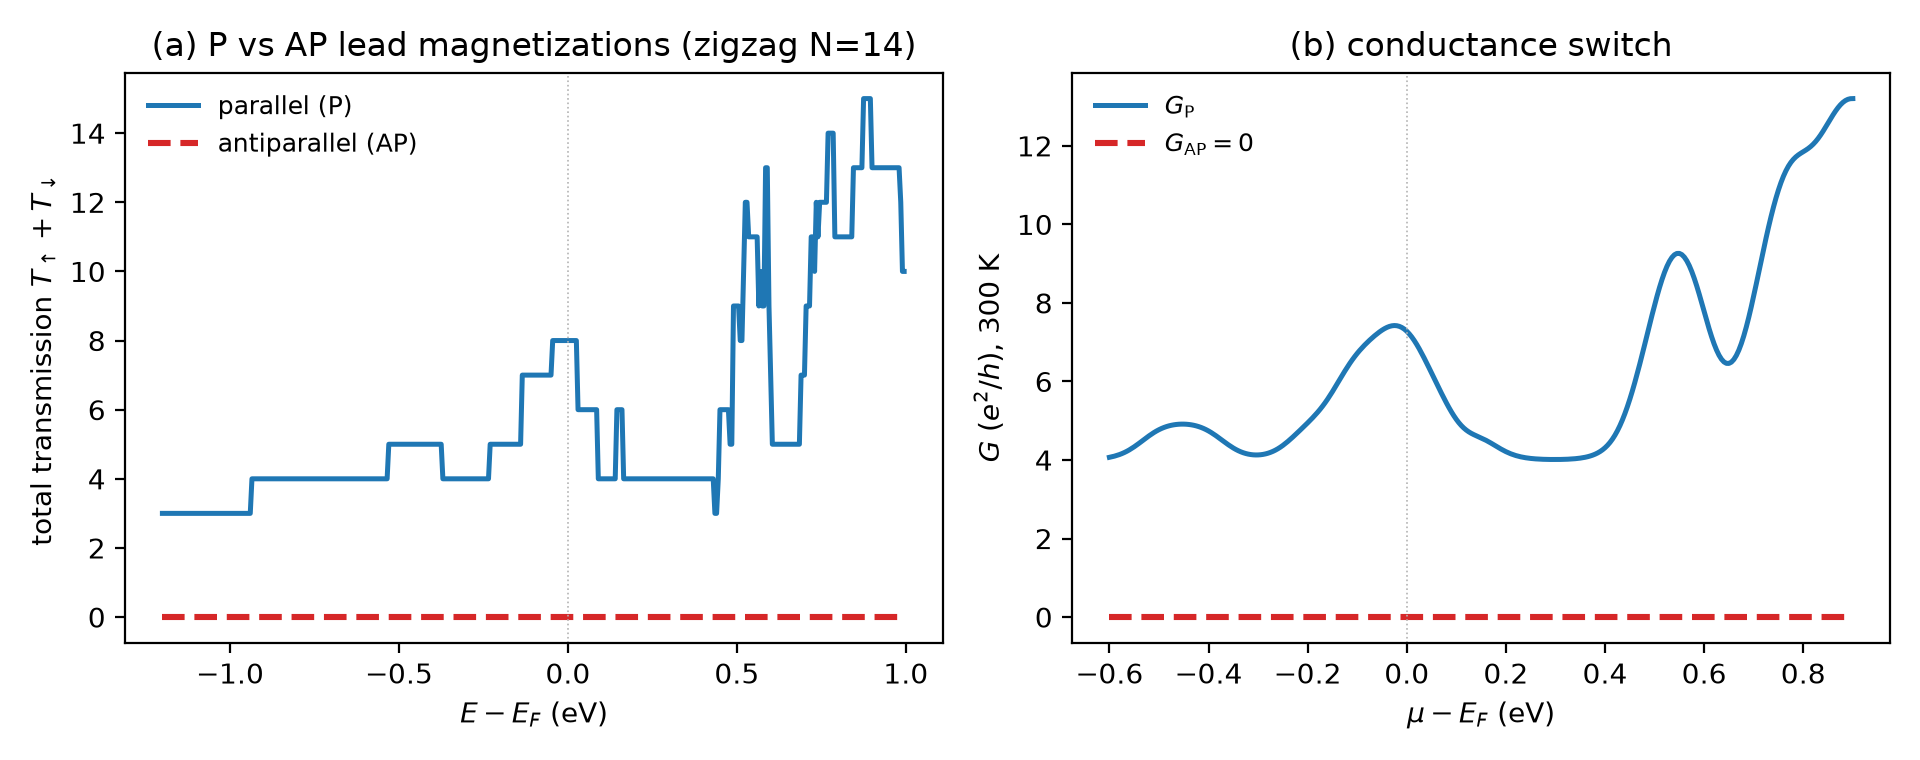
\includegraphics[width=\columnwidth]{fig_spinvalve.png}
\caption{Thermal spin valve (zigzag $N=14$). (a) Total transmission for parallel (P) and
collinear antiparallel (AP) magnetizations of the two leads: in the AP configuration each spin
species has no propagating states in one of the leads, so $T_{\rm AP}(E)=0$ identically across
the half-metallic window (displayed range $[-1.2,+1.0]$~eV; the zero was verified numerically
over the full window $[-3.2,+1.0]$~eV). (b) The resulting conductance switch at $300$~K; the
thermocurrent switches off identically.}
\label{fig:valve}
\end{figure}

\begin{figure}[t]
\centering
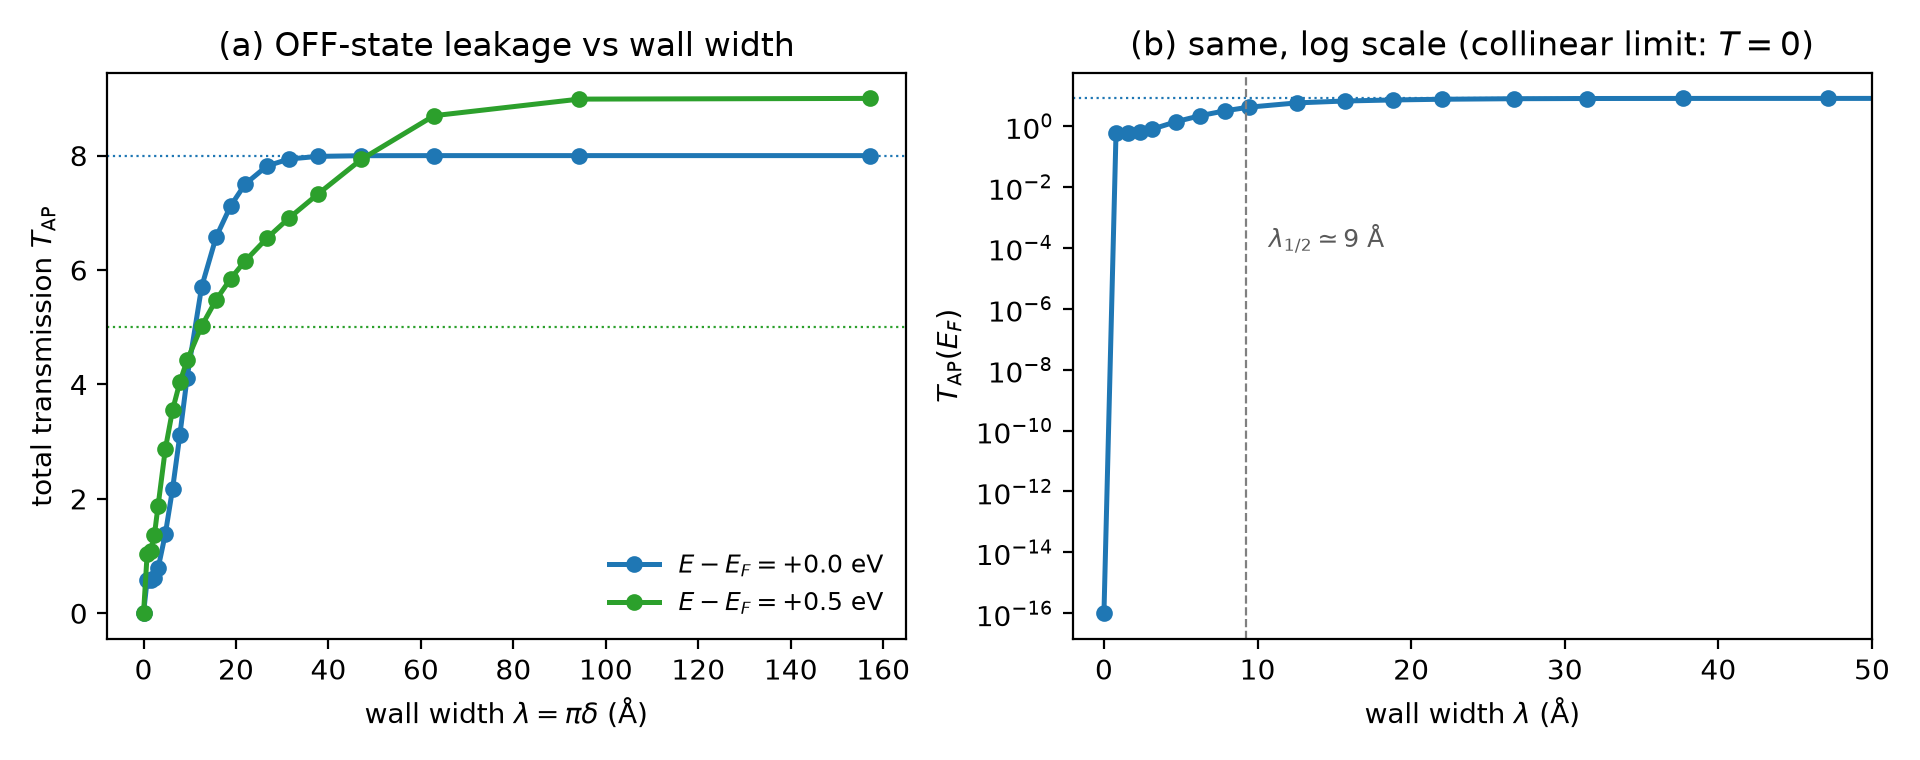
\includegraphics[width=\columnwidth]{fig_wall.png}
\caption{Domain-wall leakage of the OFF state (spinful noncollinear calculation, zigzag
$N=14$). (a) Antiparallel transmission versus wall width $\lambda$ at $E_F$ and at
$+0.5$~eV; dotted lines mark the parallel-configuration values reached in the adiabatic
(wide-wall) limit. (b) Same at $E_F$ on a log scale: the exact zero exists only at the
collinear point $\lambda=0$; the sharpest finite texture ($\lambda\simeq1$~\AA) already
transmits $T_{\rm AP}\simeq0.6$ (ON/OFF $\sim$$10$), and $\lambda_{1/2}\simeq9$~\AA\ marks
half transparency. The exact OFF state therefore requires a junction with no continuous
texture: a geometrically constrained wall~\cite{Bruno1999} or a nonmagnetic
spacer~\cite{Modarresi2019}.}
\label{fig:wall}
\end{figure}

\subsection{Edge magnetism}
\label{sec:edgemag}
Although the transport above uses the uniform bulk exchange, the same model reproduces the
magnetic edges that motivate this system. Solving the self-consistent mean-field problem of
Sec.~2.2 for the ribbon yields the per-site Cr moment profile of Fig.~\ref{fig:edgemag}. The
interior recovers the bulk moment ($2.63\,\mu_B$ in the reduced manifold, cf.\ $2.67\,\mu_B$
for the monolayer), while the reduced-coordination edge Cr atoms carry enhanced moments: by
$+4.8\%$ and $+6.1\%$ on the two inequivalent zigzag edges (the ribbon terminates on an N row
on one side and a Cr row on the other) and by $+8.3\%$ on the two equivalent armchair edges.
The enhancement is width-independent (identical for $N=14$ and $N=20$), which confirms it as
a genuine edge effect. This is the microscopic counterpart, from a lightweight model, of the
magnetic CrN nanoribbon edges analyzed by DMRG~\cite{CrNdmrg2023}. The intra-edge exchange
constants were also extracted via the magnetic-force theorem~\cite{Liechtenstein1987},
implemented with the ribbon Green's function on the real-axis contour
$E\in[-8~\mathrm{eV},E_F]$ ($400$ energies, broadening $\eta=20$~meV, $120$ $k$ points, the
perturbation acting on the three retained Cr $d$ orbitals; the script is part of the
repository). For the zigzag edge they are $J_1=+59$~meV and $J_2=+0.8$~meV (unit-vector
convention, $J>0$ ferromagnetic). The ferromagnetic $J_1$, consistent with the ferromagnetic
edge being the stable self-consistent solution, reproduces the sign of the dominant DMRG
coupling, and the strong hierarchy $|J_1|\gg|J_2|$ reproduces its qualitative structure
($J_1\simeq10$--$12$, $J_2\simeq-2$--$0$~meV/Cr~\cite{CrNdmrg2023}). The agreement is only
semi-quantitative, as expected of an analytic model with no ab-initio input: the reduced
manifold overestimates $J_1$ by a factor of $\sim$5 and gives the small $J_2$ the opposite
sign. The armchair edge shows an almost vanishing intra-edge coupling ($|J_1|<1$~meV), which
reflects the larger Cr--Cr spacing ($\sqrt3\,a$) along that edge.

\begin{figure}[t]
\centering
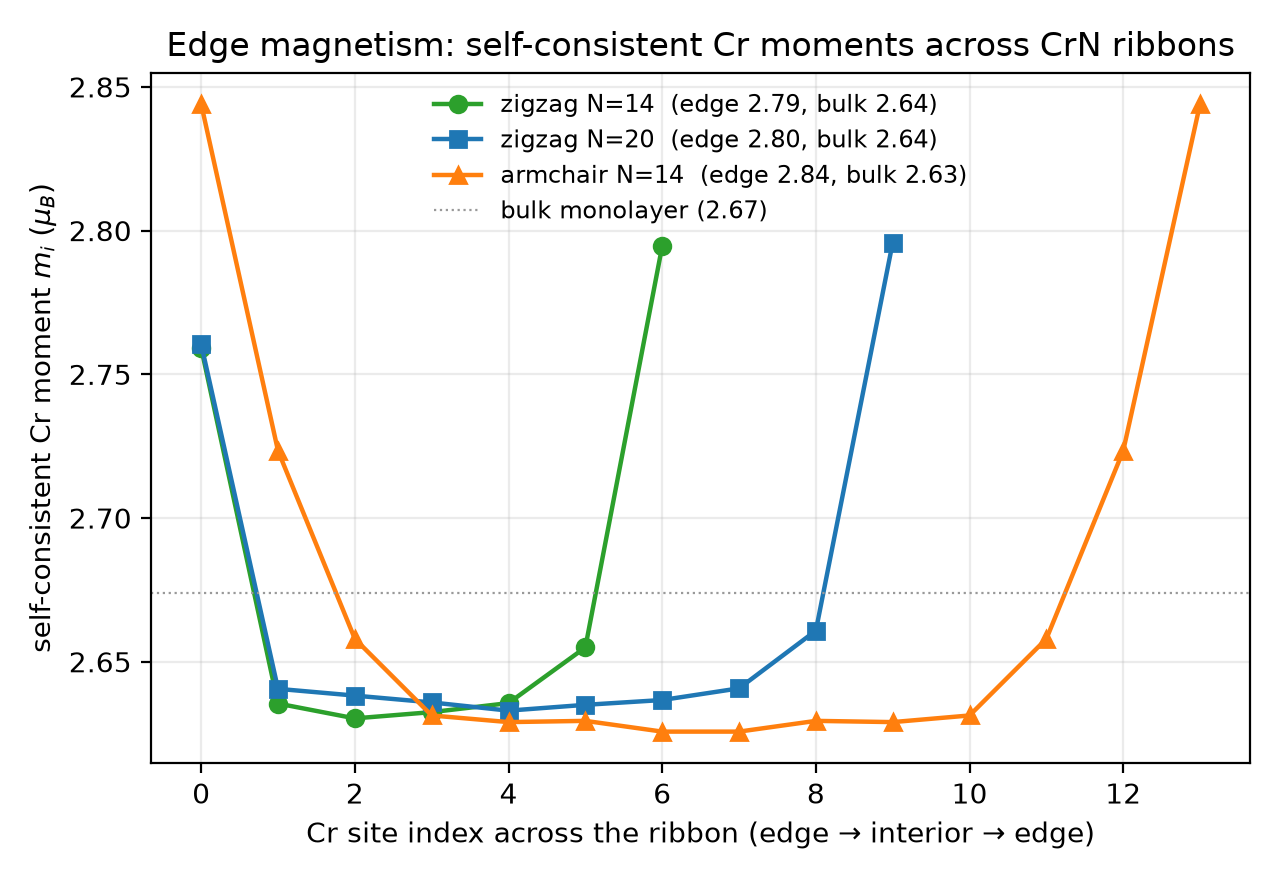
\includegraphics[width=0.82\columnwidth]{fig_edgemag.png}
\caption{Self-consistent mean-field Cr magnetic moment across the ribbon width. The interior
recovers the bulk monolayer moment (dotted line) while the reduced-coordination edge Cr atoms
carry enhanced moments: $+4.8\%$/$+6.1\%$ on the two inequivalent (N- and Cr-terminated)
zigzag edges, $+8.3\%$ on the armchair edges; the enhancement is width-independent ($N=14$ vs
$20$).}
\label{fig:edgemag}
\end{figure}

\subsection{Scope and limitations}
\label{sec:scope}
The limitations are as follows. First, the tight-binding parameters are fitted to a
published band structure (digitization uncertainty $0.1$--$0.3$~eV), so the results are
semi-quantitative. Varying every model parameter by $\pm10\%$
(Fig.~\ref{fig:sensitivity}) moves the peak $ZT$ of the zigzag $N=14$ ribbon between $0.029$
and $0.114$ about the baseline $0.063$ (for the armchair $N=8$ optimum the same protocol gives
the spread quoted in Sec.~\ref{sec:widths}). The order of magnitude
($ZT\sim10^{-2}$--$10^{-1}$) and the qualitative landscape (a modest multichannel background
inside the fully polarized window and a dominant peak at the onset of the second conduction
band) are robust, whereas individual peak heights are not converged beyond a factor of
$\sim$2; the largest excursions come from $\Delta_{\rm ex}$, from the second-shell hopping
$t_{c22}$ of the second conduction orbital, which sets the position of that band's onset, and
from $V_{pd\pi}$. The $\pm10\%$ variation is a uniform convention, not a propagated error bar:
for the on-site energies it corresponds to $0.2$--$0.35$~eV, comparable to the digitization
uncertainty, but for $\varepsilon_{c_1}$ it is only $\pm0.12$~eV and for the weakest hoppings
a few meV, smaller than their real uncertainties, and correlated variations along the
least-squares covariance are not explored.
The one parameter outside the sweep, the minority shift $\Delta^c_\downarrow$ of the effective
conduction orbitals (assumed equal to $\Delta_{\rm ex}$), has no effect: varying it by $\pm10\%$
leaves every optimum of the zigzag $N=14$ and armchair $N=8$ ribbons unchanged to four digits,
because the minority replicas lie above $+3.3$~eV, far outside the transport window.
The $\pi^*$-pinned variant of Sec.~\ref{sec:results} is our targeted probe of the one known
systematic misfit, and, as emphasized in Sec.~\ref{sec:caution}, no such check can detect a
missing band. Second, the $\pi^*$ valence band disperses incorrectly, a $0.19$~eV error in
energy as well as a misplacement in $k$ (Sec.~\ref{sec:results}); the pinned variant of
Sec.~\ref{sec:widths} is the targeted probe of this systematic. The two effective conduction
orbitals reproduce the majority conduction bands only up to $\simeq2.8$~eV, the top of the
traced range (Sec.~\ref{sec:methods}). Third, $\kappa_{\rm ph}$ is a coherent ballistic estimate
anchored to the published phonon dispersion (Sec.~\ref{sec:phonons}); anharmonicity and edge
roughness would reduce it and raise $ZT$, which is why we bracket it, and the
phonon-engineering route to $ZT$ enhancement~\cite{Sevincli2010} requires phonon transport
through the disordered geometry itself (Sec.~\ref{sec:te}). Fourth, the transport uses the uniform bulk exchange; the self-consistent edge moments differ
by only $5$--$8\%$, so feeding the site-dependent exchange back into the transmission is a
small refinement we omit. Fifth, all transport assumes saturated ferromagnetic order
with a temperature-independent exchange splitting. The random-phase-approximation estimate of
the ordering temperature of the freestanding monolayer is $T_C\simeq209$~K (Hubbard $U=3$~eV;
$124$~K at $U=0$)~\cite{Modarresi2019}, and the finite-temperature order of the ribbon edges
has been analyzed by DMRG~\cite{CrNdmrg2023}; results at and above room temperature therefore
presuppose that magnetic order survives (stabilized, e.g., by a substrate or anisotropy), and
the $ZT(T)$ curves up to $700$~K in Fig.~\ref{fig:designrules} should be read as
ordered-phase transport with $\Delta_{\rm ex}(T)$ softening neglected. A related caveat is
that phase coherence itself is an idealization at high temperature: electron--phonon
dephasing shortens the coherent mean free path well before $700$~K in a real device, so the
$ZT(T)$ trend above room temperature is best read as the coherent-transport projection rather
than a quantitative prediction for a partially incoherent device at those temperatures.
Finally, transport at $\mu-E_F\simeq+1$~eV assumes a rigid band structure under heavy
electron doping or gating, an approximation that a self-consistent treatment of screening
would refine.

\begin{figure}[t]
\centering
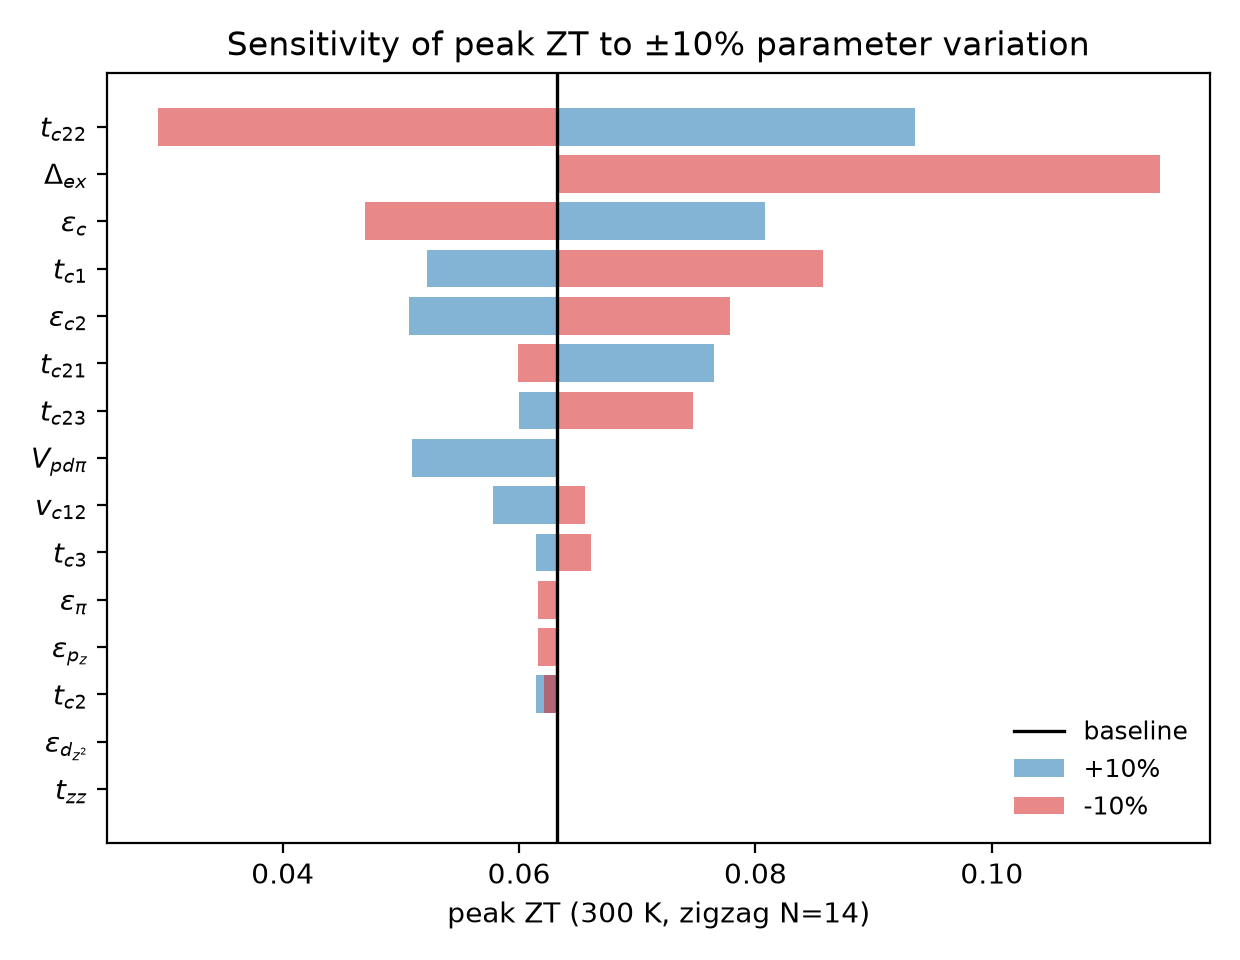
\includegraphics[width=0.85\columnwidth]{fig7_sensitivity.png}
\caption{Sensitivity of the peak figure of merit (zigzag $N=14$, $300$~K, global optimum) to a
$\pm10\%$ variation of each model parameter, including those of the effective conduction
orbitals. The spread is $[0.029,0.114]$ about the baseline $0.063$: the order of magnitude is
robust; individual peak heights are semi-quantitative. The $\pm10\%$ variation is a uniform
convention, not a propagated error bar (see text).}
\label{fig:sensitivity}
\end{figure}

%% ------------------------------------------------------------------
\section{Conclusions}
\label{sec:conclusions}

We have presented, to our knowledge, the first thermoelectric-transport study of hexagonal CrN
nanoribbons, using a tight-binding plus Landauer approach parametrized entirely from published
first-principles data. The paper makes four claims. (i)~As thermoelectrics, pristine CrN
nanoribbons are modest: $ZT\simeq0.06$--$0.15$ at $300$~K across widths and edges
($\kappa_{\rm ph}$ brackets in Table~\ref{tab:results}). Once both majority conduction bands
are resolved, every global optimum lies inside the fully spin-polarized window, at the onset
of the second conduction band ($\mu-E_F\simeq+0.5$--$0.7$~eV) for five geometries and on the
hole-doped side for the narrow armchair $N=8$ ribbon, which has the best figure of merit,
$ZT=0.15$ $[0.08$--$0.24]$ (Fig.~\ref{fig:armchair8}); the minority edge is never the
optimum, and this landscape is unchanged by the model's one known systematic misfit.
(ii)~As spin filters they are outstanding: the minority channel is gapped over nearly
$4$~eV. The half-metallicity itself, however, confirms the first-principles and semiclassical
predictions~\cite{Kuklin2017,CrNdmrg2023}; what this work adds is its phase-coherent
quantification (quantized, $100\%$-polarized transmission across the accessible window, robust
in width and edge type) and the coincidence of the thermoelectric optimum with full
polarization.

(iii)~The same gap powers a thermally driven spin valve with an \emph{exact} collinear OFF
state. The noncollinear domain-wall calculation shows that any continuous magnetization
texture leaks (half transparency already at $9$~\AA). The published exchange and
anisotropy values place the intrinsic wall width at $2.4$--$3$~nm, where the wall is at least $95\%$
transparent and reaches the exact adiabatic limit at the upper end of that range;
geometrically constrained or spacer-separated junctions are therefore required, not merely preferred. (iv)~Methodologically, the minimal
orbital manifold suggested by the states at $E_F$ fabricates a sharp band edge and a fivefold
overestimate of $ZT$ ($0.33\to0.063$ for the zigzag $N=14$ ribbon). The
artifact is invisible to parameter-sensitivity analysis, a concrete caution for minimal-basis
nanoribbon thermoelectric studies in general. Supporting these claims, the self-consistent
mean-field treatment reproduces the magnetic edges and, semi-quantitatively, the dominant
exchange coupling's sign and its hierarchy over the sub-leading one found by DMRG.

%% ------------------------------------------------------------------
\section*{CRediT authorship contribution statement}
\textbf{Tomas Rojas:} Conceptualization, Methodology, Software, Validation, Investigation,
Writing -- original draft, Writing -- review \& editing. \textbf{Ruhi Thorat:} Validation,
Writing -- review \& editing.

\section*{Declaration of competing interest}
The authors declare that they have no known competing financial interests or personal
relationships that could have appeared to influence the work reported in this paper.

\section*{Funding}
This research did not receive any specific grant from funding agencies in the public,
commercial, or not-for-profit sectors.

\section*{Data and code availability}
The tight-binding/transport code (Python, Kwant), the digitized reference data (band-structure
and phonon anchors) and the scripts that generate all figures and tables are openly available
in the accompanying repository,\\
\url{https://github.com/tomas0821/crn-nanoribbon-thermoelectric},\\
where a tagged release records the exact version used to produce the numbers in this
manuscript.

%% ------------------------------------------------------------------
\bibliographystyle{elsarticle-num}
\bibliography{refs}

\end{document}
